
\documentclass[a4paper,UKenglish,cleveref, autoref, thm-restate]{lipics-v2021}

\bibliographystyle{plainurl}% the mandatory bibstyle
\usepackage{booktabs}   %% For formal tables:
                        %% http://ctan.org/pkg/booktabs
\usepackage{subcaption} %% For complex figures with subfigures/subcaptions
                        %% http://ctan.org/pkg/subcaption

\usepackage{mathtools}
\usepackage{todonotes}
	\usepackage{microtype}

	\usepackage{complexity}
	 \usepackage{amsmath}
\usepackage{dsfont}

	\usepackage{stmaryrd}
\usepackage{MnSymbol}
\usepackage{graphicx}




\newcommand{\problemx}[3]{
	\vspace{0.2cm}
\par\noindent\underline{\sc#1}\par\nobreak\vskip.2\baselineskip
\begingroup\clubpenalty10000\widowpenalty10000
\setbox0\hbox{\bf INPUT:\ }\setbox1\hbox{\bf QUESTION:\ }
\dimen0=\wd0\ifnum\wd1>\dimen0\dimen0=\wd1\fi
\vskip-\parskip\noindent
\hbox to\dimen0{\box0\hfil}\hangindent\dimen0\hangafter1\ignorespaces#2\par
\vskip-\parskip\noindent
\hbox to\dimen0{\box1\hfil}\hangindent\dimen0\hangafter1\ignorespaces#3\par
\endgroup
	\vspace{-0.2cm}
}

\newcounter{claimcounter}
\setcounter{claimcounter}{0}
\newtheorem{subclaim}{Subclaim}{}
\newtheorem{fact}{Fact}{}
\newtheorem*{theorem*}{Theorem}

\makeatletter

\usepackage{ textcomp } 

\usepackage{stmaryrd}
\usepackage{MnSymbol}
\usepackage{graphicx}

\usepackage{wrapfig}



\renewcommand{\poly}{\mathrm{poly}}


\newcommand{\alain}[1]{\todo[inline,color=red!20]{{\bf AF:} #1}}
\newcommand{\mathieu}[1]{\todo[inline,color=blue!20]{{\bf MH:} #1}}



\title{Decidability of Resilience for WSTS} 

\titlerunning{Resiliency} 

\author{Alain Finkel}
{Université Paris-Saclay\and CNRS\and ENS Paris-Saclay\and Laboratoire Méthodes Formelles (LMF)\and Gif-sur-Yvette, France}
{finkel@lsv.fr}{}{This work was partly done while the author was supported by the Agence Nationale de la Recherche grant no. (numero de la grant BraVASS).}

\author{Mathieu Hilaire}
{Université Paris-Saclay\and CNRS\and ENS Paris-Saclay\and Laboratoire Méthodes Formelles (LMF)\and Gif-sur-Yvette, France}{hilaire@lsv.fr}{}{This work was partly done while the author was supported by the Agence Nationale de la Recherche grant no. (numero de la grant BraVASS).}

% \authorrunning{M. Hilaire}

\Copyright{M. Hilaire} 


\ccsdesc{Theory of computation~Automata over infinite objects}
\ccsdesc[500]{Theory of computation~Automata extensions}

\keywords{}



\category{} 

\relatedversion{}
% \relatedversiondetails{Full Version}{}

\acknowledgements{The author would like to thank.}


\ArticleNo{70}
\begin{document}

\maketitle


\begin{abstract}
	Here goes the abstract.
\end{abstract}


\newcommand{\LCM}{\mathsf{LCM}}
\newcommand{\LOGSPACE}{\mathsf{LOGSPACE}}
\newcommand{\MSO}{\mathsf{MSO}}
\newcommand{\SO}{\mathsf{SO}}

 \newcommand{\N}{\mathds{N}}



	\section{Introduction}\label{section introduction}


{\bf Context.} 
Resilience is a key notion for improving safety of unperfect systems and resilience engineering is a paradigm for safety management that focuses on systems coping with complexity and balancing productivity with safety~\cite{challenges}. Some systems are subjects at frequent intervals to accidents, attacks or changes. Think for instance of a supply chain, or an airport’s air trafic control. In such cases, a question that arises is that of whether the system can return to its normal (safe) behavior after an accident or attack
pushed it towards some kind of ‘error state’ and, if it can, whether it can perform the return in a satisfactory timeframe. 
%%%%%%%%
%\alain{fait double emploi avec l'exemple si on le développe ce que je ne suis plus sûr...:  In the exemple of air trafic control, an accident i.e. for instance a delay in the arrival of a plane can lead to conflicts of resolution (i.e. landing) which lead to prompting planes to remain on standby. Since their fuel quantity is limited it is hence pretty important to be able to know that trafic will return to its normal pace quickly enough. We formalize this as the resilience problem. 
%Resilience is then the capacity of a system that fall in a bad set of states to leave this set and to reach a safe set of states. \\
%
%State-resilience only consider bad elements that are reachable from an initial state, while bounded-resilience and $k$-resilience ask whether safe is reachable in a bounded number of step and $k$ or less steps respectively.}


{\bf Home-spaces}
 In 1986, Memmi and Vautherin introduced the notion of home-space~\cite{DBLP:conf/ac/MemmiV86} for a system $\mathscr{S} = (S,\rightarrow )$ with an initial state $s_0$ : a subset $H \subseteq S$ is an \emph{home-space}  if 
%			from all reachable states from $s_0$, it is always possible to reach $H$ 
$\post^*(s_0) \subseteq \pred^*(H)$; it could be easily generalized for two subsets $X,H$ and we say that $H$ is an \emph{home-space for $X$} if $\post^*(X) \subseteq \pred^*(H)$. In 1989, de Frutos Escrig and Johnen proved that the home-space problem (for $X$ a singleton and $H$ a finite union of linear sets with the same period) was decidable for VASS (only published as an internal report). In 2023, Jancar and Leroux proved the decidability of the (complete) semilinear home-space problem ($X$ and $H$ are both semilinear)  in VASS \cite{DBLP:journals/corr/abs-2207-02697}.
%%%%%

{\bf Resiliences.}  
The (general) resilience property for a transition system $\mathscr{S} = (S,\rightarrow )$ and a subset of states $\Safe \subseteq S$ consists of the following: $\mathscr{S}$ is {\em $\Safe$-resilient} if
$S \subseteq \pred^*(\Safe)$. %In the case 
% it
It 
can be stated as an home-space problem : $\mathscr{S}$ is $\Safe$-resilient if $\post^*(S) \subseteq \pred^*(\Safe)$.
Similarly, $\mathscr{S}$ is $\Safe$-state-resilient for an initial state $s_0$ if  
$\post^*(s_0) \subseteq \pred^*(\Safe)$.
We will study three decidability questions for each of type of resilience.
The resilience problem is to decide whether a transition system $\mathscr{S} = (S,\rightarrow )$ is $\Safe$-resilient (for a given subset of states $\Safe \subseteq S$).
The resilience problem could be easily generalized for two subsets $\Bad$ and $\Safe$ by asking
whether $\Bad \subseteq \pred^*(\Safe)$.
The $k$-resilience problem is to decide whether $S \subseteq \pred^{\leq k}(\Safe)$ (for a given $k$) and 
the bounded resilience problem is to decide whether there exists an $k$ such that $\mathscr{S}$ is $\Safe$-$k$-resilient. We adapt these three definitions to state-resilience.


{\bf State of the art.}
In 2016, Prasad and Zuck introduced in  \cite{DBLP:journals/corr/PrasadZ16} interesting definitions and results (without detailed proofs) about resilience in the framework of process algebra. They built the composition of the process and its adversary as a transition system and they gave conditions that insure that the composed transition system is an effective WSTS with both upward and reflexive downward compatibilities (and some other technical conditions). In this framework and under these hypotheses, resilience reduces to coverability which is decidable on WSTS. 
%Since the definition of resilience is only given informally in the introduction as "a process is resilient to an adversary if its observable behaviour in the presence of adversarial action is equivalent to its behaviour in the absence of the adversary", it still remains unclear what is formally resilience.
%%%%%%%%%

In 2021, Ozkan and Würdemann  \cite{DBLP:journals/corr/abs-2108-00889} and Okzan \cite{DBLP:conf/gg/Ozkan22}, in 2022, proved the decidability of the bounded state-resilience problem and the $k$-state-resilience problem for WSTS  with strong compatibility and with the supplementary (strong) hypothesis that there exists an algorithm that computes a finite basis of $\uparrow \post^*(s)$ for all state $s$ (called effective 
$\uparrow$ $\post^*$ basis) and with $\Safe=\uparrow \Safe$ and $\Bad$ downward-closed.
%		(even though \cite{DBLP:conf/gg/Ozkan22} also discuss, albeit briefly, the other possible cases). 
%		The paper of Prasad and Zuck \cite{DBLP:journals/corr/PrasadZ16} is not quoted by Ozkan and Würdemann.

Remark that the reflexive downward compatibility (of an effective WSTS) hypothesis in  \cite{DBLP:journals/corr/PrasadZ16} implies the existence of an algorithm that computes a finite basis of $\uparrow \post^*(s)$ for all state $s$; this provides a way to use \cite{DBLP:journals/corr/abs-2108-00889} for proving the announced result by Prasad and Zuck.
However, neither Prasad \& Zuck nor Ozkan \& Würdemann established the strong relation between resilience and the home-space property.
%%%%%%%%%
%





% {\bf FSTTCS 2033  Submission deadline: July 14, 2022 AoE (firm) Notification to authors: September 16, 2022}

% trop d'hypotheses trop fortes sur les WSTS
\noindent
{\bf Our contributions}
\begin{itemize}
%\item We investigate and expand upon the notion of state-resilience ~\cite{DBLP:journals/corr/PrasadZ16,DBLP:journals/corr/PrasadZ16,DBLP:journals/corr/abs-2108-00889,DBLP:conf/gg/Ozkan22} and we study three decidability questions for each of type of resilience. We remark that it is an instance of the home-space problem~\cite{DBLP:journals/corr/abs-2207-02697,memmi2023invariants}.

\item Surprinsingly, the general undecidability statements about resilience were not known neither proved. We show that resilience and { State-resilience} problems are both undecidable for WSTS with strong compatibility. 
% \alain{harminiser les notations des pbs { State-resilience} ou  State-resilience ?}
% \mathieu{je pense dans l'intro on peut conserver State-resilience et par contre une fois le probleme de {\ State-resilience} proprement défini c'est cette notation qu'il faudrait utiliser}
%Moreover, state-resilience,
%bounded-state-resilience and
% $k$-state-resilience
%are undecidable for WSTS with strong compatibility having an effective pred-basis. 
Moreover, { State-resilience},
{ Bounded-state-resilience} and
{ $k$-state-resilience}
are undecidable for strongly upward-compatible WSTS with effective pred-basis
when
$\Safe=\uparrow \Safe$. We made a reduction of zero-reachability in reset-VASS to {\ State-resilience} in reset-VASS.


\item The three resilience problems are decidable for completion-post-effective $\omega^2$-WSTS with strong compatibility and $\Safe = \uparrow \Safe$.


\item The resilience problem is decidable for ideal-effective WSTS with 
$\Safe=\downarrow \Safe$
and
the additional hypothesis that
for all downward-closed set $D \subseteq S$, the set $\pred^*(D)$ is downward-closed.
%
%%%

\item We generalize the main theorem of \cite{DBLP:journals/corr/abs-2108-00889,DBLP:conf/gg/Ozkan22} by relaxing the strong compatibility hypothesis.
%: {\ State-resilience} is still decidable for 
% WSTS with effective 
%$\uparrow$ $\post^*$ basis
%when
%$\Safe=\uparrow \Safe$
We also show that removing the effective 
$\uparrow$ $\post^*$ basis hypothesis leads to undecidability. We extend and prove the main result in  \cite{DBLP:journals/corr/PrasadZ16} : the three state-resilience problems are decidable for ideal-effective WSTS with downward and upward compatibilities ({ $k$-state-resilience} and { bounded-state-resilience} are decidable for ideal-effective WSTS with strong downward compatibility).
%

\item We study the resilience problems for VASS and variations of VASS where most of the resilience problems are shown decidable.
\end{itemize}


 \begin{center}
	\begin{figure}
	%		\hspace{3cm}
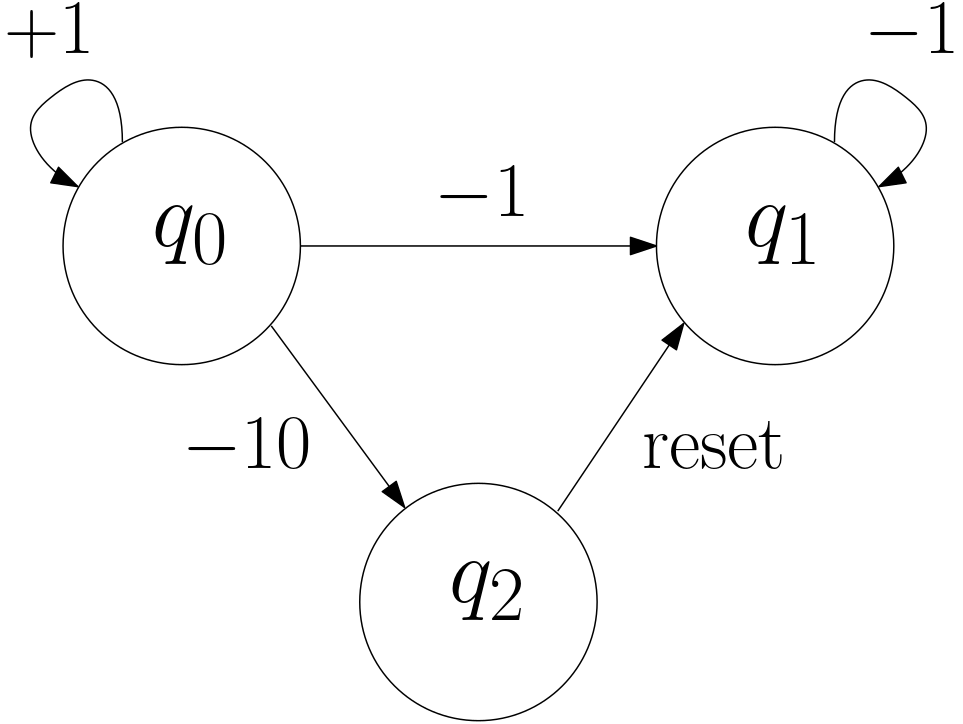
\includegraphics[width=0.4\textwidth]{FigureC}
\hspace{0.6cm}
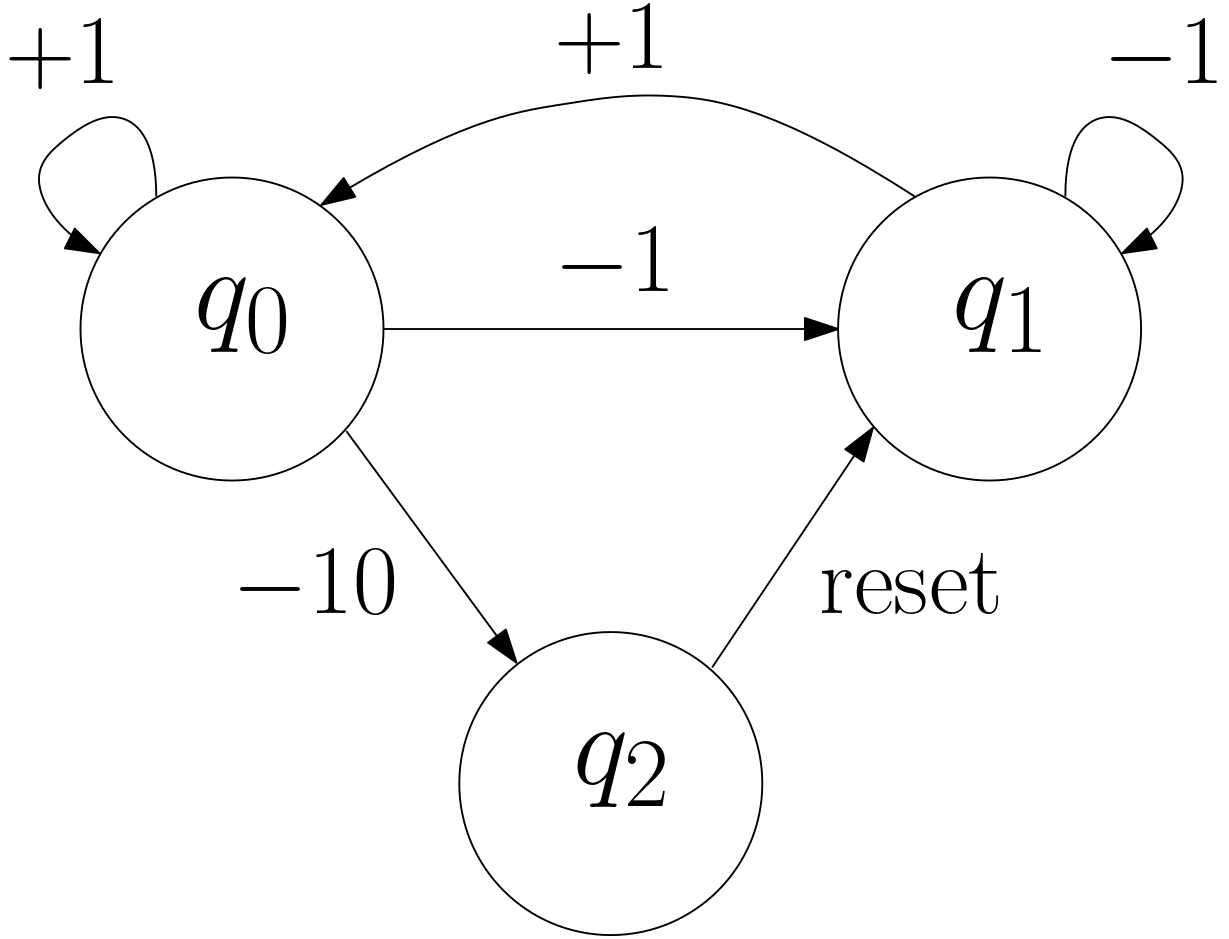
\includegraphics[width=0.4\textwidth]{FigureD}
	\caption{Two reset-VASS with three states and one counter.}
					\label{r-V}
	\end{figure}
\end{center}

\begin{example}\label{Example}
{(\bf Reset-VASS example).}
Consider the leftmost reset-VASS from Figure~\ref{r-V}.
Consider first $\Safe = \{q_0(n) \mid n \in \N\}$; In this case,  {Resilience}, { $k$-resilience} and { Bounded resilience} are not satisfied: there is no  way back from $q_2$ or $q_1$ to $q_0$. Consider now $\Safe = \{q_1(0)\} $; then { Resilience} hold: it is possible to reach $q_1(0)$ from any configuration of $V$. However, { Bounded resilience} do not hold, since, for all $n\in \N$, from $q_1(n)$, there is no path of lenght less than $n$ towards $q_1(0)$. Consider now the rightmost reset-VASS, which corresponds to having added a $+1$ transition from $q_1$ back to $q_0$. In this reset-VASS { Bounded resilience} hold, since $6$-resilience hold. 
Indeed, from any configuration with value of the counter bigger than $9$, it is possible to reach $q_2$ in two steps or less, then use the reset transition. From $q_1(n)$ or $q_0(n)$ with $n \in \{1, 2, 3, 4, 5, 6\}$ it is possible to reach $q_1(0)$ in $6$ steps or less. From 
$q_1(n)$ or $q_0(n)$ with $n \in \{7,8\}$ it is possible to reach $q_0(10)$ in $3$ steps or less, from which $q_1(0)$ is reachable in $2$ steps.
\end{example}



\newcommand{\pred}{\textsf{pred}}
\newcommand{\post}{\textsf{post}}
% \renewcommand{\succ}{\textsf{Succ}}

\section{Definitions}\label{section definitions}



In this section, we introduce general notations and preliminary definitions.

The model we are interested in is WSTS (and later some particular instances, i.e. Timed/Counter Automata for instance).


% \textcolor{red}{Before defining WSTS, need a definition of TS and WQO}


\subsection{Transition systems}


\begin{definition}
An {\em transition system} is a pair $\mathscr{S} = (S,\rightarrow )$ where $S$ is a set of 
{\em states} and  
$ {\rightarrow} \subseteq S \times S$ is a
binary relation 
on
the set of states, denoted as the set of {\em transitions}. A {\em labeled transition system} (LTS for short) is a tuple $\mathscr{S}=(S, \Sigma, \rightarrow)$ where 
$S$ is a set of {\em states}, $\Sigma$ is a (finite) set of {\em labels}, and 
${\rightarrow} \subseteq S\times \Sigma \times S$ is a 
ternary relation,
denoted as the set of {\em labeled transitions}. 
\end{definition}

Note 
 that an (unlabeled) transition system can be seen as a labeled transition system where the set of labels consists of only one element. 

We again prefer to use infix notation and write $s \rightarrow s'$ to denote a {\em transition} from state $s$ to state $s'$ (i.e., $ (s,s') \in  {\rightarrow} $). \newline

%
\alain{enlever ce qui est inutile}
%
Determinism, (infinite) paths, their length, and concatenation in unlabeled transition systems are
then defined as expected.

%\textcolor{red}{Thinking about whether or not it is pertinent to have LTS and not only TS. LTS can be usefull for TA because of the use of the guards/time as labels but it may be unecessary.}

We write $\rightarrow^{k}$, $\rightarrow^{+}$, $\rightarrow^{=}$, $\rightarrow^{*}$
for the $k$-step iteration of $\rightarrow$, its transitive closure, its reflexive closure, its reflexive and transitive closure). We use similar notation for $\post$ and $\pred$...

Let $X,Y \subseteq S$ and $k \in \mathbb{N}$. We denote $X \longrightarrow^{*} Y$ (resp. $X \longrightarrow^{\leq k} Y$) if from all states $x \in X$ there exists a path (resp. of length smaller than $k$) that reaches a state $y \in Y$.

%\textcolor{red}{This makes sense for TS but not so much for LTS ...}

A transition system is {\em finitely branching} if all $\post(s)$ are finite. 
%\textcolor{blue}{We restrict our attention to finitely branching TSs.}

%\textcolor{blue}{Alain: the forward coverability algorithm for infinitely branching TSs.; the backward cov algo may work for essentially finitely branching TSs.}
%\textcolor{red}{Not sure that TS induced by TA are finitely branching. Actually I believe they are not, i.e. for instance for a TA with one clock $x$, from a state $q$ and clock $x$ set at $0$, if there is a transition e.g. $(q, x \geq 3, \emptyset, q')$ then the set of successors of 
%$(q,0)$ is $\{q'\} \times \{3, 4, 5, \ldots \}$. Need to check where finitely branching appears as an assumption/requirement.}

%
%\begin{definition}
%A {\em labeled transition system} (LTS for short) is a tuple $\mathscr{S}=(S, \Sigma, \rightarrow)$ where 
%$S$ is a set of {\em states}, $\Sigma$ is a (finite) set of {\em labels}, and 
%${\rightarrow} \subseteq S\times \Sigma \times S$ is a 
%ternary relation,
%denoted as the set of {\em labeled transitions}. 
%\end{definition}

We
 prefer to use infix notation and $(s,a ,s')\in {\rightarrow} $ will be abbreviated as
       $s  \xrightarrow{a}  s'$
to represent a transition from configuration $s$ to configuration $s'$ with label $a$. \\

\noindent
%Labels can be used to represent the reading of an input, but also to represent an action performed during the transition or conditions that must hold in order to allow the use of the transition.


A {\em path} in a labeled transition system from a {\em source configuration} $s_0$
to a {\em target configuration} $s_n$ is a sequence 
$\pi = s_0 \xrightarrow{a_0 } s_1 \xrightarrow{a_1 } \cdots \xrightarrow{a_{n-1} } s_n$.

We define the {\em concatenation} $ \pi_1 \pi_2$ of 
two paths $\pi_1$ and $\pi_2$ when the source configuration of $\pi_2$ is equal to the target configuration of $\pi_1$
as expected.
The {\em length} of 
$\pi = s_0 \xrightarrow{a_0 } s_1 \xrightarrow{a_1 } \cdots \xrightarrow{a_{n-1} } s_n$
is defined as $|\pi|=n$ and we say the path is {\em labeled} by $a_0 a_1 , \ldots a_{n-1}$.
For all $w \in \Sigma^*$, all $s,s' \in S$, we will write $s \xrightarrow{w } s'$ if there exists a path from $s$ to $s'$ labeled by $w$. 

An {\em infinite path} is an infinite sequence
 $\pi = s_0 \xrightarrow{a_0 } s_1 \xrightarrow{a_1 } \cdots $.
For each infinite (resp. finite) path  $\pi = s_0 \xrightarrow{a_0 } s_1 \xrightarrow{a_1 } \cdots$ 
(resp. $\pi = s_0 \xrightarrow{a_0 } s_1 \xrightarrow{a_1 } \cdots \xrightarrow{a_{n-1}} s_n$)
and $i,j \in \N$ (resp. $i,j \in [0,n]$) with $i<j$ we denote
by $\pi[i,j]$ the path 
$s_i  \xrightarrow{a_i } s_{i+1}  \xrightarrow{a_{i+1} } \cdots  \xrightarrow{a_{j-1} } s_j$
 and by $\pi[i]$ the configuration $s_i$.
As expected, a {\em prefix} of a finite or infinite path $\pi$ is a finite path of the form $\pi[0,j]$, and
a  {\em suffix} of a finite path $\pi$ is a path of the form $\pi[i,n]$.  \\
Given an infinite path $\pi = s_0 \xrightarrow{a_0 } s_1 \xrightarrow{a_1 } \cdots$ let
$\text{\textit{Inf}}(\pi) = \{ s \in S \mid \forall i ~ \exists j > i ~ s_j = s\}$.



\noindent
The set of {\em (immediate) successors} of a state $s \in S$ is defined as
$\post(s) = \{ s' \in S \mid \exists a \in \Sigma ~ s \xrightarrow{a} s'\}$.
A state without successors is called a {\em dead end}.  \\
The set of {\em (immediate) predecessor} of a state $s \in S$ is defined as
$\pred(s) = \{ s' \in S \mid \exists a \in \Sigma ~ s' \xrightarrow{a} s\}$.



A labeled transition system $(S, \Sigma, \rightarrow)$ is {\em deterministic} if for all states $s_1, s_2, s_3 \in S$ and all
$a \in \Sigma$,
 $ s_1  \xrightarrow{a} s_{2}$ and  
 $s_1  \xrightarrow{a} s_{3} $ implies $s_2 = s_3 $. \\

%
\alain{enlever ce qui est inutile}
%


\subsection{Well-quasi-orderings}

A {\em quasi-ordering} (a qo) is any reflexive and transitive relation $\leq$ over some set $X$ and we often write $(X,\leq)$.

We abbreviate $x \leq y \not\leq x$ by $x < y$.

% A partial ordering (a po) is an antisymmetric qo

Any qo induces an equivalence relation ($x \equiv y$ iff $x \leq y \leq x$).
% and gives rise to a po between the equivalence classes ?
% 	do we need po ?

We now recall a few results from the theory of well-orderings (add reference [...]).


\begin{definition}
 A {\em well-quasi-ordering} (a wqo) is any quasi-ordering $(X,\leq)$ such that, for any infinite sequence $x_0, x_1, x_2, ...$ in $X$, there exist indexes $i \leq j$ with
$x_i \leq  x_j$.
\end{definition}


There exists a stronger formulation. $(X,\leq)$ is a wqo iff any infinite sequence  $x_0, x_1, x_2, ...$ in $X$ contains an infinite increasing subsequence: $x_{i_0} \leq x_{i_1} \leq x_{i_2} \cdots$ (with $i_0 < i_1 < i_2 \cdots$).

% \textcolor{red}{Add lemma about infinite increasing subsequences ?}
%
\iffalse
%
\begin{lemma}
(Erd\"os and Rado). Assume $\leq$ is a wqo. Then any infinite sequence contains an infinite increasing subsequence: $x_{i_0} \leq x_{i_1} \leq x_{i_2} \cdots$ (with $i_0 < i_1 < i_2 \cdots$).
\end{lemma}


\begin{proof}
Consider an infinite sequence and the set $M = \{i \in N \mid \forall j > i ~ x_i \not\leq x_j \}$. $M$ cannot
be infinite, otherwise it would lead to an infinite subsequence contradicting the wqo
hypothesis. Thus, $M$ is bounded and any $x_i$ with $i$ beyond $M$ can start an infinite
increasing subsequence.
\end{proof}
%
\fi
%

Given $(X,\leq)$ a quasi-ordering, an {\em upward-closed set} is any set $U \subseteq X$ such that if $y \geq x$ and $x \in U$ then $y \in U $.
A {\em downward-closed set} is any set $D \subseteq X$ such that if $y \leq x$ and $x \in D$ then $y \in D $. 
To any subset $A \subseteq X$, we may associate
its {\em upward-closure},
 $\uparrow A = \{x \in X \mid \exists a \in A ~ y \geq a\}$
 and its 
 {\em downward-closure},
 $\downarrow A = \{x \in X \mid \exists a \in A ~ y \leq a\}$. 
We abbreviate $\uparrow \{x\}$ (resp. $\downarrow \{x\}$)
as $\uparrow x$ (resp. $\downarrow x$).


A {\em basis} of an upward-closed set $I$ is a set $I_b$ such that $I = \uparrow I_b$. 
% Higman investigated ordered sets with the finite basis property.

Wqo admits many other equivalent formulations. For instance: 
$(X,\leq)$ is a wqo if and only if any infinite increasing sequence $U_0 \subseteq U_1 \subseteq U_2 \subseteq \cdots$ of
upward-closed subsets in $X$ eventually stabilizes, 
%      i.e. there is a $k \in N$ such that $U_k = U_{k+1} = U_{k+2} = \cdots $ 
if and only if any upward-closed subset $U \subseteq X$ has a
finite basis if and only if $(X,\leq)$ is well-founded (i.e. it admits no infinite strictly decreasing sequence) and $X$ don't contain infinite subset of mutually incomparable elements (antichains).
%
\iffalse
%

\begin{lemma}{(Higman [40])} 
If $\leq$ is a wqo then any upward-closed $I$ has a
finite basis.
\end{lemma}

% \textcolor{red}{Expliquer ce que c'est une base d'abords.}

\begin{proof}
The set of minimal elements of $I$ is a basis because $\leq$ is well-founded. It
only contains a finite number of non-equivalent elements otherwise they would make
an infinite sequence contradicting the wqo assumption.
\end{proof}



\begin{lemma}  \label{upward-closed stablizes}
If $\leq$ is a wqo then any infinite increasing sequence $I_0 \subseteq I_1 \subseteq I_2 \subseteq \cdots$ of
upward-closed sets eventually stabilizes, i.e. there is a $k \in N$ such that 
$I_k = I_{k+1} = I_{k+2} = \cdots $.
\end{lemma}

\begin{proof}
Assue we have a counter-example.
We extract an infinite subsequence where
inclusion is strict: $I_{n_0} \subsetneq I_{n_1} \subsetneq I_{n_2} \cdots$. Now, for any $i>0$, we can pick some $x_i \in I_{n_i} \setminus I_{n_{i-1}}$. The well-quasi-ordering hypothesis means that the infinite sequence of $x_i$'s
contains an increasing pair $x_i \leq x_j$ for some $i<j$. Because $x_i$ belongs to an upward-
closed set $I_{n_i}$ we have $x_j \in I_{n_i} $, contradicting $x_j \not\in I_{n_{ j - 1}}$.
\end{proof}
%
\fi
%

Quasi-orderings that have no infinite antichains enjoy a similar \emph{finite decomposition} property than wqo. In such \emph{Finite Antichains} sets $(X,\leq)$, every downward closed subset $D \subseteq X$ can be decomposed into a \emph{finite} set of ideals $J_i$ (an ideal is a directed downward closed subset): $D = \downarrow (J_1 \cup J_2 \cup..\cup J_n)$.

In what follows, a downward closed set is represented by its finite set of ideals 
%		$D=\downarrow D$   $I_D=\{J_1, J_2,...,J_n\}$ 		satisfying $D = \downarrow (J_1 \cup J_2 \cup..\cup J_n)$ 
and an upward closed set $U$ is represented by its finite set minimal elements.
% $M_U$ of its  satisfying $U=\uparrow M_U$.

\alain{est-ce utile et correct ? Let $I,J$ be two upward-closed sets given by its set of minimal element and $D,E$ be two downward-closed sets given by its ideal decomposition. All the four  inclusions $U \subseteq V$,  $U \subseteq D$, $D \subseteq U$ and $D \subseteq E$ are decidable provided that the ordering is decidable.}

% \textcolor{red}{Define WSTS}

% \textcolor{red}{Define SWSTS -  necessary}

\subsection{Well-structured transition systems}


\begin{definition}\cite{DBLP:journals/iandc/Finkel90,DBLP:journals/tcs/FinkelS01}
A {\em (resp. strongly) well-structured transition system} (abbreviated as WSTS)  $(S, \rightarrow, \leq)$
is a transition system $(S, \rightarrow)$
equipped with a wqo ${\leq} \subseteq S \times S$ between states such that  
%  decidable ≤  wqo on S, i.e., for each two given states s, s ′ ∈ S, it is decidable whether s ≤ s ′ . 
the transition relation $ \rightarrow$ is compatible (resp. strongly compatible) with the wqo, i.e., for all 
$s_1, t_1 , s_2 \in S$
	with $s_1 \leq s_2$  and $s_1 \rightarrow t_1$ , there exists 
	$t_2 \in S$ with 
	$t_1 \leq t_2$ and $s_2 \rightarrow^{*} t_2$ 			
				(resp. $s_2 \rightarrow t_2$ ).
\end{definition}

Several families of formal models of processes give rise to WSTSs in a natural way, e.g. Petri nets when inclusion between markings is used as the well-ordering.


% \textcolor{red}{Define 'has effective pred-basis'. Maybe it should be included in WSTS definition, maybe it can be another def. I kind of like the idea of 'effective pred-basis' and 'decidable $\leq$' being independant from the WSTS definition}
\iffalse
\begin{proposition}\cite{DBLP:journals/tcs/FinkelS01}
If $\mathscr{S}$ is an WSTS and $U \subseteq S$ is an upward-closed set of states, then $\pred^*(U )$ is upward-
closed.
\end{proposition}
%
Proof. Assume $s \in \pred^* (U )$. Then $s \rightarrow^* t$ for some $t \in U $. If now $s' \geq s$ then upward-compatibility entails that $s' \rightarrow^* t'$ for some $t' \geq t$. Then $t' \in U$ and $s' \in \pred^*(U )$.
\fi

\begin{proposition}\cite{DBLP:journals/tcs/FinkelS01}
If $\mathscr{S}$ is a WSTS with strong compatibility and $U \subseteq S$ is upward-closed, then $\pred(U )$, $\pred^k(U )$ and $\pred^*(U )$ are upward-closed.
\end{proposition}
%\alain{étrange ces deux propositions, l'une suffirait}
\iffalse
Proof. Assume $s \in \pred (I )$. Then $s \rightarrow t$ for some $t \in I $. If now $s' \geq s$ then strong upward-compatibility entails that $s' \rightarrow t'$ for some $t' \geq t$. Then $t' \in I$ and $s' \in \pred(I )$.

\mathieu{On peut probablement enlever la Proposition $8$ alors. La proposition $9$ étant plus directement pertinente pour les lemmes/preuves (permet d'avoir itérativement $\pred^k(I)$ upward-closed if $I$ upward-closed - for all $k$).}
\fi


\begin{definition}\cite{DBLP:journals/tcs/FinkelS01,DBLP:journals/iandc/AbdullaCJT00}
A WSTS $\mathscr{S}$ has {\em effective pred-basis} if there exists an algorithm accepting
any state $s \in S$ and returning $pb(s)$, a finite basis of $\uparrow \pred(\uparrow s)$.
\end{definition}

% \textcolor{red}{Define what an Ideal is. Actually an Ideal is just an upward-closed set, so maybe this just adds some confusion. Anti-ideal just downward closed so again just not that helpful a notation. Maybe have a }


\iffalse
\begin{definition}
A {\em bi-ideal} $I \subseteq S$ is an upward-closed and downward-closed set, i.e
$\uparrow I = I = \downarrow I$.
\end{definition}

"Bi-ideals often represent “control states” as in [cf \%]. "
% Parosh Aziz Abdulla, Karlis Cerans, Bengt Jonsson & Yih-Kuen Tsay (1996): General Decidability Theorems for Infinite-State Systems. In: Proc. LICS 1996, IEEE Computer Society Press, pp. 313–321,

% \textcolor{red}{Probably one can already 'deduce' from this that ideal $I$ and anti-ideal $J$ for resp. good and bad states, in the case of e.g. timed automata would be given by sets of states}
\fi

A downard-closed set $D$ is {\em decidable} if, given $s \in S$, it is decidable whether
$s \in D$. 
%\textcolor{red}{Since a downward-closed set does not have an ``upward-basis'' in general, we will demand that membership is decidable.}
% \textcolor{red}{Do we still demand this ?}
%\mathieu{On peut enlever ce point de discussion ici et en discuter de manière plus complête au moment où on discute de SAFE et BAD plus en détail je pense.}

\begin{claim}{(stability of upward-closed sets)}
Let $U, V \subseteq S$ be upward-closed. Then the sets $U \cup V$, and $U \cap V$ are upward-closed.
\end{claim}


% \begin{claim}
% Given a finite set $A \subseteq S$ with $I =\uparrow A$, we can compute a finite basis $B$ of $I$.
% \end{claim}

\begin{fact}\label{fact basis}
% Fact 3 ([1]). 
% Parosh Aziz Abdulla, Karlis Cerans, Bengt Jonsson & Yih-Kuen Tsay (1996): General Decidability Theorems for Infinite-State Systems. In: Proc. LICS 1996, IEEE Computer Society Press, pp. 313–321,
For every upward-closed set $U \subseteq S$, there exists a finite basis $B$ of $U$. 
% (ii) Given a finite set $A \subseteq S$ with $I =\uparrow A$, we can compute a finite basis $B$ of $I$.
% \alain{(ii) est bizarre car A est déjà une base finie de $\uparrow A$, et $min(A)$ est la base minimale}
\end{fact}


\begin{definition}{ (index)}. 
If $\mathscr{S}$ is a WSTS with strong compatibility and $U \subseteq S$  is upward-closed and $k \geq 0$, let $U^k= \bigcup_{0 \leq j \leq k} \pred^j(U)$.
The {\em index} $k(U)$ is the
smallest $k_0$ s.t. $U^k = U^{k_0}$ for all $k \geq k_0$.
\end{definition}


If $\mathscr{S}$ is a WSTS with strong compatibility and $U \subseteq S$ is an upward-closed set, the sets $\pred(U )$, and $\pred^{\geq k}(U )$ for
every $k \geq 0$ are upward-closed, thus Lemma~\ref{upward-closed stablizes} ensures the existence of $k(U)$.

\begin{remark}
$U^{k+1} $ can be rewritten $U^{k+1}= \bigcup_{0 \leq j \leq k+1} \pred^j(U) = 
U \cup \bigcup_{1 \leq j \leq k+1} \pred^j(U) =
U \cup \pred(\bigcup_{0 \leq j \leq k} \pred^j(U))
=  U \cup \pred(U^k)$.
\end{remark}

This ensures the following.

\begin{fact}\label{stop condition}
% Fact 4 (stop condition). 
If $\mathscr{S}$ is a WSTS with strong compatibility and $U \subseteq S$ is an upward-closed set and $k \geq 0$ s.t. $U^k = U^{k+1}$ , then $U^\ell = U^k$ for all $\ell \geq k$, i.e.,
$k(U) \leq k$. This also implies that $\pred^*(U) = U^k$.
\end{fact}


\begin{lemma}
% Lemma 3 ([1]) 
% Parosh Aziz Abdulla, Karlis Cerans, Bengt Jonsson & Yih-Kuen Tsay (1996): General Decidability Theorems for Infinite-State Systems. In: Proc. LICS 1996, IEEE Computer Society Press, pp. 313–321,
 Given a basis of an upward-closed set $U \subseteq S$, and a state $s$ of an effective strongly WSTS, we can decide whether $U  \xrightarrow {*}{} s$.
%	we can reach $U$ from $s$.
\end{lemma}

\begin{proof}
We have to show that we can compute a basis of $U^{k+1}$ if we are given a basis of $U^k $. 
Then the
decidability of the stop condition follows directly. Let $B$ be a basis of $U^k$. 
We have
$$U^{k+1} = U \cup \pred(U^k ) = U \cup
\bigcup_{s' \in B}
\pred(\uparrow \{s' \}).$$

Since a finite basis of $\pred(\uparrow \{s' \}$) is computable for any $s'\in S$ by definition, we obtain a finite generating set of $U^{k+1}$ . By
Fact~\ref{fact basis}, we can compute a basis of $U^{k+1}$.
\end{proof}

\begin{theorem}
A finite basis of $ \pred^*(U)$ is computable for any effective WSTS $\mathscr{S}$ with effective pred-basis and any upward closed set $U \subseteq S$ given with its finite basis $B_U$.
\end{theorem}




%%%
\iffalse
%%%%
%%%%
\subsection{Defining resilience}


\subsubsection{Resilience for general transition systems}

% \textcolor{red}{Ask the question why use a set of propositions for $SAFE$ and $BAD$ rather than use subsets of the set of configurations ? }

We ask whether we can reach a state 
%which satisfies
in 
%
$SAFE$  in a reasonable amount of time whenever we reach a state 
% which satisfies
in
%
$BAD$. 
From this we formulate two resilience problems. First consider the case where the recovery time
is bound by a given natural number $k \geq 0$, i.e., the \emph{explicit resilience problem} for TS.

\problemx{$k$-Resilience problem }
{a transition system $(S,\rightarrow)$, an integer $k$, a state $s \in S$, $SAFE, BAD \subseteq S$ and $SAFE \cap BAD = \emptyset$.}
{$\forall s' \in BAD, ~ s \rightarrow^* s' \implies \exists s'' \in SAFE ~ s' \rightarrow^{\leq k} s''$ ?\newline}

If a system $S$ satisfies the explicit resilience property for an integer $k$, we say that $S$ is $k$-resilient.

% If we assume that the transition system yields infinite sequences of transitions, we can express the property to be evaluated in CTL by s |= AG(BAD → 0≤ j≤k EX j SAFE). 

We can also ask whether there exists such a bound $k$ such that $S$ is $k$-resilient. We call this problem the \emph{bounded resilience problem}.

%
%\problemx{Bounded Resilience problem}
%{a transition system $(S,\rightarrow)$, a state $s \in S$, $Safe, BAD \subseteq S$ and $Safe \cap BAD = \emptyset$.}
%{$\exists k \geq 0 ~ \forall s' \in BAD, ~ s \rightarrow^* s' \implies \exists s'' \in Safe ~ s' \rightarrow^{\leq k} s''$ ?\newline}
%


\problemx{Bounded Resilience problem}
{a transition system $(S,\rightarrow)$, a state $s \in S$, $Safe, Bad \subseteq S$ and $Safe \cap Bad = \emptyset$.}
{$\exists k \geq 0  \mathscr{S}$ is $k$-resilient. ?\newline}
%%

%%%


pour $k,k'$ donnés, chercher si $Safe_{max}$ et $Bad_{max}$ ont un sens ? on peut faire l'union des Safe, Safe' et des Bad, Bad' prendre le max des k. Fixer k, chercher et calculer $Safe_{max}$ et $Bad_{max}$.

%
%\alain{dire juste que Safe = upward closed et BAD = downward closed.
%envisager les 3 autres cas. souvent BAD = upward closed (par ex l'exclusion mutuelle).
%4 resilience problem (U,D), (U,U), (D,U), (D,D)}

\fi



\section{Resilience for WSTS}


The resilience problem (resp. the $k$-resilience problem) in a transition system is to decide whether from a bad state, there exists a path (resp. a path of length smaller than $k$) that reaches a Safe state. Let us formalize these properties.

\problemx{resilience problem (RP)}
{A transition system $\mathscr{S}=(S,\rightarrow)$ and two sets $Safe, Bad \subseteq S$.}
{$Bad \longrightarrow^{*} Safe$ ?\newline}
%
%\alain{il faudrait ne pas répéter 3 fois les mêmes imputs pour les 3 pbs: énoncer les 3 uniformes pbs d'un coup avec une fois l'input puis les 3 pbs pour un état s donné sans répéter non plus 3 fois les mêmes inputs}

\problemx{$k$-resilience problem (kRP)}
{A transition system $\mathscr{S}=(S,\rightarrow), k \in \mathbb{N}$ and two sets $Safe, Bad \subseteq S$.}
{$Bad \longrightarrow^{\leq k} Safe$ ?\newline}

We add a third problem that decides whether there exists an $k$ such  that the system is $k$-resilient.
%
\problemx{bounded resilience problem (BRP)}
{A transition system $\mathscr{S}=(S,\rightarrow)$ and two sets $Safe, Bad \subseteq S$.}
%{$\exists k \geq 0 ~ \forall s' \in D ~ s \rightarrow^* s' \implies \exists s'' \in U ~ s' \rightarrow^{\leq k} s''$ ?\newline}
{$\exists k \geq 0$ such that $\mathscr{S}$ is %uniformely
 $k$-resilient ?\newline}

\alain{trouver les Bad et Safe maximum tels que S est resilient. est-ce vrai que si S est $(B_i,D_i)$-resilient alors S est $(\cap, \cup B_i,D_i)$-resilient ? on pourrait décider que Safe=complement de Bad et donc on aurait un seul ensemble (et son complement)}

These three reachability problems are decidable for finite transition systems but undecidable for (general) infinite-state transition systems. 
So we restrict our framework to the class of infinite-state WSTS. Since most of decidable properties in WSTS are given as effective upward or downward closed sets \cite{DBLP:journals/iandc/AbdullaCJT00, DBLP:journals/tcs/FinkelS01}, we consider upward closed or downward closed sets Safe and Bad.
\alain{on peut penser à des ensembles Bad definis dans une logique booleennne sur les clos par le bas, haut, +...}

For instance, the well-known mutual exclusion property is often modelized in a $d$-counters machine by the property that a counter $c_{mutex}$ must be bounded by (usually) one. Then, the set $Safe =  \{c_{mutex} \leq 1\} \times \mathbb{N}^{d-1}$ is downward closed and $Bad =\{c_{mutex} \geq 2\} \times  \mathbb{N}^{d-1} $ is the upward closed complementary of Safe. In \cite{DBLP:conf/gg/Ozkan22}, the authors considered that Bad is always downward closed and Safe is always upward closed.
%		
RP is decidable for lossy counter machines (LCM) with Safe and Bad semilinear sets as a consequence of results in Section 3.4 of \cite{DBLP:conf/rp/Schnoebelen10}. In particular, the existing proofs of resilience use the decidability of reachability; but we wish to decide resilience for models with undecidable reachability.
%
In what follows, we will always suppose that a downward closed set $D$ is given by its finite set of ideals $I_D=\{J_1, J_2,...,J_n\}$ satisfying $D=\downarrow D = \downarrow (J_1 \cup J_2 \cup..\cup J_n)$ and that an upward closed set $U$ is given by its finite set $Min_U$ of its minimal elements satisfying $U=\uparrow Min_U$.

Let $U,V$ be two upward-closed sets given by its set of minimal element and $D,E$ be two downward-closed sets given by its ideal decomposition. All the four  inclusions $U \subseteq V$,  $U \subseteq D$, $D \subseteq U$ and $D \subseteq E$ are decidable provided that the ordering is decidable and sets are recursive.
%
\alain{on peut penser à des ensembles bad definis dans une logique booleennne sur les clos par le bas, haut, +...}


\begin{proposition}\label{general}
$\mathscr{S}=(S,\rightarrow,\leq)$ is %uniformely 
(bad,Safe)-resilient iff $bad \subseteq \pred^*(Safe)$.\\
$\mathscr{S}=(S,\rightarrow,\leq)$ is %uniformely 
(bad,Safe)-bounded-resilient iff $\mathscr{S}=(S,\rightarrow,\leq)$ is %uniformely 
(bad,Safe)-resilient.\\
$\mathscr{S}=(S,\rightarrow,\leq)$ is %uniformely 
(bad,Safe)-$k$-resilient iff $bad \subseteq \pred^k(Safe)$.
\end{proposition}

\begin{proof}
Resilient means that 
\end{proof}


\subsection{Case: $Safe=\uparrow Safe$.}


\begin{theorem}\label{up-down}
The three %uniform 
resilience problems are decidable for WSTS with effective predbasis and $Safe=\uparrow Safe$.
%	and bad is upward closed or downward closed.
\end{theorem}


\begin{proof}
Let us first solve if $\mathscr{S}=(S,\rightarrow,\leq)$ is %uniformely 
(bad,Safe)-resilient. Since $Safe=\uparrow Safe$, and WSTS, $\pred^*(Safe)=\uparrow \pred^*(Safe)$, so $\pred^*(Safe)$ admits a finite basis $B_{\pred^*(Safe)}$. since WSTS  with effective predbasis, we may compute a finite basis of $\pred^*(Safe)$ with the backward coverability algorithm. 
%Then if bad is upward closed or downward closed, we may decide the inclusion $Bad \subseteq \uparrow B_{\pred^*(Safe)}$ which remais to compare, in both cases, two finite sets. 
if bad  is upward closed, $bad = \uparrow B_{bad}$ and $ \uparrow B_{bad} \subseteq \uparrow B_{\pred^*(Safe)}$ iff for every $b \in B_{bad}$, there is a $s \in B_{\pred^*(Safe)}$ such that $s \leq b$. similar reasonning for the other case.
hence the two %uniform
 resilience problems are decidable.

Let us examine the %uniform 
$k$-resilience problem (kRP). we may compute the least $n$ such that $bad \subseteq \uparrow \pred^n(Safe)=  \uparrow \pred^*(Safe)$. $S$ is %uniformely 
$k$-resilient iff $n \leq k$ \alain{hum...mais il peut y avoir des chemins plus courts}and then kRP is decidable.
\end{proof}

%One begins to test whether $Bad \cap \pred^*(Safe) = \emptyset$ then never resilient car une fois dans bad j'y reste sans pouvoir aller dans Safe.\\

If $Bad \cap \pred^*(Safe) \neq \emptyset$, One computes the minimal elements $A$ of $Bad \cap \pred^*(Safe)$.
resilient iff $Bad \subseteq \pred^*(Safe)$  (eq $Bad \cap \pred^*(Safe) = Bad$)

$Bad \cap \pred^*(Safe) \neq Bad$ alors, on peut se limiter à $Bad' = Bad \cap \pred^*(Safe)$ et c'est (Bad',Safe)-resilient.

Let us show that the predbasis hypothesis can be replaced by other hypotheses.

\subsection{Case: $Safe=\uparrow Safe$ and $BAD=\downarrow BAD$.}

%
%		cas étudié par les deux articles sur les graphes
%


%  Parosh Aziz Abdulla, Karlis Cerans, Bengt Jonsson & Yih-Kuen Tsay (1996): General Decidability Theorems for Infinite-State Systems. In: Proc. LICS 1996, IEEE Computer Society Press, pp. 313–321,
%  Alain Finkel & Philippe Schnoebelen (2001): Well-structured transition systems everywhere! Theor. Comput. Sci. 256(1-2), pp. 63–92, doi:10.1016/S0304-3975(00)00102-X.

%Transfering the abstract resilience problems into this framework,
%it is therefore reasonable to demand that both propositions, Safe and BAD, are given by 
%upward-closed or downward-closed sets.

The \emph{completion}  \cite{BFM-ic17} of a WSTS $\mathscr{S}=(S,\rightarrow, \leq)$ is the associated ordered transition system $\hat{\mathscr{S}}=(Ideals(S),\rightarrow, \subseteq)$ where states of $\hat{\mathscr{S}}$ are ideals of $S$ and $I \rightarrow J$ if $J$ belongs to the finite ideal decomposition of $\downarrow \post_{\mathscr{S}}(I)$. The completion is always finitely branching but it is not necessarly WSTS since $\subseteq$ is not necessarly a wqo. $\hat{\mathscr{S}}$ is WSTS iff $\mathscr{S}=(S,\rightarrow, \leq)$ is $\omega^2$-WSTS (intuitively speaking, $(S,\leq)$ must not contain the Rado set). Coverability is shown decidable  [Theorem 44] in \cite{BFM-ic17} for completion-post-effective $\omega^2$-WSTS.

Let us recall two other results in \cite{BFM-ic17}. Proposition 30 establishes a strong relation between the runs of a WSTS $\mathscr{S}=(S,\rightarrow, \leq)$ and the runs of its completion $\hat{\mathscr{S}}$. It states that if $x \xrightarrow{k} y$ in $\mathscr{S}$ then for every ideal $I \supseteq \downarrow x$, there exists an ideal $J \supseteq \downarrow y$ such that $I \xrightarrow{k} J$ in $\hat{\mathscr{S}}$. Proposition 29 establishes that if $I \xrightarrow{k} J$ in $\hat{\mathscr{S}}$ then for every $y \in J$, there exists $x \in I$ and $y' \geq y$ such that $x \xrightarrow{k'} y'$ in $\mathscr{S}$. Moreover, if $\mathscr{S}$ has transitive compatibility then $k’ \geq k$; if $\mathscr{S}$ has strong compatibility then $k’ = k$.


\begin{proposition}\label{down-up}
Let $\mathscr{S}=(S,\rightarrow, \leq)$ be a completion-post-effective $\omega^2$-WSTS with strong compatibility and two finite sets: $I_{BAD}$ and $Min_{Safe}$.
The %uniform 
resilience problem (RP) and the %uniform 
bounded resilience problem (BRP) are decidable.
The %uniform
 $k$-resilience problem (kRP) is decidable if moreover $\mathscr{S}$ has the predbasis hypothesis.
\end{proposition}

\begin{proof}
Let $I_{BAD}=\{J_1, J_2,...,J_n\}$ be the ideal decomposition of $BAD$ and $B_{Safe}=\{b_1,b_2,...,b_m\}$ be the minimal basis of $Safe$.
The %uniform 
resilience problem (RP) is equivalent to an infinite number of instances of the coverability problem : for all $x \in BAD$ does there exist an $j$ such that $b_j$ is coverable from $x$. This infinite set of coverability questions can be reduced to $n$ instances of the coverability problem in the completion $\hat{\mathscr{S}}=(Ideals(S),\rightarrow, \subseteq)$ of $\mathscr{S}=(S,\rightarrow, \leq)$.

%Proposition 30 in \cite{BFM-icalp14} establishes a strong relation between the runs of a WSTS $\mathscr{S}=(S,\rightarrow, \leq)$ and the runs of its completion $\hat{\mathscr{S}}$. It states that if $x \xrightarrow{k} y$ in $\mathscr{S}$ then for every ideal $I \supseteq \downarrow x$, there exists an ideal $J \supseteq \downarrow y$ such that $I \xrightarrow{k} J$ in $\hat{\mathscr{S}}$. Proposition 29 establishes that if $I \xrightarrow{k} J$ in $\hat{\mathscr{S}}$ then for every $y \in J$, there exists $x \in I$ and $y' \geq y$ such that $x \xrightarrow{*} y'$ in $\mathscr{S}$.

Let us show that $b_j$ is coverable from $x$ in $\mathscr{S}$ iff $\downarrow b_j$ is coverable (for inclusion) from $\downarrow x$ in $\hat{\mathscr{S}}$.

Suppose that $b_j$ is coverable from $x$ then there exists a run $x \xrightarrow{k} y \geq b_j$. From Proposition 30, there exist an ideal $J$ and a run $\downarrow x \xrightarrow{k} J$ where $J \supseteq \downarrow y \supseteq \downarrow b_j$ in $\hat{\mathscr{S}}$, hence $b_j$ is covered from $\downarrow x$.
Conversely, if $I \xrightarrow{k} J$ in $\hat{\mathscr{S}}$ with $\downarrow b_j \subseteq J$ then 
%	for every $y \in J$, 
there exists $x \in I$ and $y' \geq b_j$ such that $x \xrightarrow{k} y'  \geq b_j$ in $\mathscr{S}$ and then $b_j$ is coverable from $x$ in $\mathscr{S}$.

%
% iff there is a run in $\hat{S}$ from an ideal I to J such that  $\downarrow x \subseteq I$ and $\downarrow b_j \subseteq J$. This is a consequence of  
%Propositions 29 and 30 in \cite{BFM-icalp14} that establish a strong relation between the runs of a WSTS $\mathscr{S}=(S,\rightarrow, \leq)$ with its completion $\hat{S}$.
%' \in I(BAD)$.

To decide the %(uniform)
 bounded resilience problem (BRP), we decide $n \times m$ coverability questions: is state $b_j$ coverable from ideal $J_i$ ? If all these $n \times m$ coverability questions are positive then we compute $K=max(k_a \mid a=1,..,m \times n)$ and we deduce that  $\mathscr{S}$ is %uniformely
  $K$-resilient. Since coverability is decidable for completion-post-effective $\omega^2$-WSTS, we have shown that both the %uniform 
  resilience problem (BRP) and the %uniform 
  bounded resilience problem (BRP) are decidable.

To decide the kRP, we may compare the input $k$ with $K$. If $k \geq K$, we conclude that is %uniformely 
$k$-resilient; if $k < K$ we cannot answer. if moreover $\mathscr{S}=(S,\rightarrow, \leq)$ has the predbasis hypothesis, we may compute the least $n$ such that $ \uparrow \pred^n(Safe)=  \uparrow \pred^*(Safe)$. $S$ is %uniformely
 $k$-resilient iff $n \leq k$ \alain{hum...mais il peut y avoir des chemins plus courts}and then kRP is decidable.
\end{proof}

%

\subsection{Case: $Safe=\uparrow Safe$ and $BAD=\uparrow BAD$.}

%%



\subsection{Case: $Safe=\downarrow Safe$ and $BAD=\downarrow BAD$.}

%%%%%%%%
\subsection{Case: $Safe=\downarrow Safe$ and $BAD=\uparrow BAD$.}
%
%		cas exclusion mutuelle
%
je prends les minimaux de bad et les idéaux de Safe, pas sur que ce soit decidable....$pred(Safe)$


\begin{tabular}{ l c r }
   BAD/Safe & Up & Down \\
   Up & dec ? & dec ? \\
   Down & dec & ? \\
 \end{tabular}

%We first assume that the safety property is given by an upward-closed set and the bad condition by a decidable downward-closed set. 
% \textcolor{red}{Seems like a reasonable assumption to me.}

%From these considerations, we formulate instances of the abstract resilience problems for well-
%structured transition systems.








\section{State-resilience}


Resilience is a strong property since it implies that from every element of $\Bad$ there must exist a path to $\Safe$. But, when one considers a system with an initial state $s_0$, it could be sufficient to ask that only from $\Bad \cap post^*(s_0)$, there must exist a path to $\Safe$. 
%
%			However, this condition seems more difficult since one also must decide whether a state $s \in \Bad$ is reachable from $s_0$.
%
%\problemx{(I,J)-$k$-resilience problem for WSTS}
%{A state $s$ of a WSTS $(S,\rightarrow, \leq)$, an effective set $I$ (with a given basis), a set $J$.}
%{$\forall s' \in J ~ (s \rightarrow^* s') \implies \exists s'' \in I ~ s' \rightarrow^{\leq k} s''$ ?\newline}
%
%\problemx{general $k$-resilience problem for WSTS}
%{A state $s$ of a WSTS $(S,\rightarrow, \leq)$, an effective set $I$ (with a given basis).}
%{$\forall s'  ~ (s \rightarrow^* s') \implies \exists s'' \in I ~ s' \rightarrow^{\leq k} s''$ ?\newline}

%		Again, we first consider the case where the recovery time is bounded by a $k \in \N$.

The three previous problems become:


\problemx{State-resilience problem (SRP)}
{A transition system $\mathscr{S}=(S,\rightarrow)$, $s \in S$ and two sets $\Safe, \Bad \subseteq S$.}
% 		an upward-closed set $\Safe$ with a given basis, a decidable downward-closed set $\Bad$.}
% 		{$ ~ \forall s' \in \Bad, ~ s \rightarrow^* s' \implies \exists s'' \in \Safe, ~ s' \rightarrow^{*} s''$ ?\newline}
{$\Bad \cap \post^*(s)  \rightarrow^{*} \Safe $ ? \newline}


\problemx{$k$-state-resilience problem (kSRP)}
{A transition system $\mathscr{S}=(S,\rightarrow)$, $s \in S$ and two sets $\Safe, \Bad \subseteq S$.}
{ $\Bad \cap \post^*(s) \longrightarrow^{\leq k} \Safe$ ?  \newline}
%

\problemx{bounded-state-resilience problem (BSRP)}
{A transition system $\mathscr{S}=(S,\rightarrow)$, $s \in S$ and two sets $\Safe, \Bad \subseteq S$.}
%{$\exists k \geq 0 ~ \forall s' \in D ~ s \rightarrow^* s' \implies \exists s'' \in U ~ s' \rightarrow^{\leq k} s''$ ?\newline}
{$\exists k \geq 0$ such that $\mathscr{S}$ is $k$-state-resilient. ?\newline}


%\textcolor{blue}{
%justification des definitions: si on enlève la condition  an upward-closed set $U$ (extended resilience $U$ qq) reachability reduces to resilience (avec $U=\{x\}$ donc indecidable pour les modèles à reachability indécidable.
%}



Since these problems are undecidable for general infinite-state transition systems, we restrict our study to WSTS.

As in the Section~3, we study decidability results for different pairs of sets $\Safe$ and $\Bad$ downward-closed and upward-closed. We will consider here the cases where 
$\Safe = \uparrow \Safe$ and $\Bad = \downarrow \Bad$ 
and where 
$\Safe = \downarrow \Safe$ and $\Bad = \uparrow \Bad$.

% \mathieu{Ici on s'intéresse seulement aux cas $\uparrow \downarrow$ et $\downarrow \uparrow$.}

\subsection{Case: $\Safe = \uparrow \Safe$ and $\Bad = \downarrow \Bad$}



Unfortunately, {\sc State-resilience} is undecidable for (general) WSTS even with strong upward-compatibility.
This stems from the fact that it is undecidable in the particular case of Reset VASS,
where  $t$-liveness is both undecidable and 
 reducible to {\sc State-resilience}.

% \noindent
% {\bf Reset VASS}

Reset VASS extend the basic VASS model with special “reset
transitions” that resets (set to $0$) some coordinates in the vector. Let us recall their definition here.\\

% More Formally {\em reset ... }



\begin{definition}
A {\em Reset VASS} in dimension $d$ (Reset $d$-VASS for short) is a finite 
% $\mathds{Z}^d$
labeled directed graph $V = (Q,T)$, where $Q$ will be referred to as the {\em control-states} of $V$, and where 
%$T \subseteq Q \times \mathds{Z}^d \times Q$
$T \subseteq Q \times Op \times Q$
 will be referred to as the {\em control-transitions} of $V$,
where $Op = \{ add(\textbf{z}) \mid \textbf{z} \in \mathds{Z}^d\} \cup 
		\{ reset(i) \mid i \in \{1,\ldots,d\} \}$.
\end{definition}

Again $Q \times \N^d$
 denotes the set of configurations of $V$.
For every configurations $p(\textbf{u}), q(\textbf{v}) \in Q \times \N^d$ and every control-transition $t$ we write
$p(\textbf{u}) \xrightarrow{t} q(\textbf{v})$ when 

\begin{itemize}

\item  $t = (q,add(\textbf{z}),q') \in T$
% then for all $\textbf{u} \in \N^d$ such that  
% $\textbf{u}+\textbf{z} \geq 0$
% $q(\textbf{u}) \xrightarrow{\textbf{z}} q'(\textbf{u}+\textbf{z})$,
and $\textbf{u}+\textbf{z} = \textbf{v} \geq 0$,

\item $t = (q,reset(\gamma),q') \in T$ 
% then for all $\textbf{u} \in \N^d$ 
% $q(\textbf{u}) \xrightarrow{z} q'(\textbf{u}')$,  where 
and
$\textbf{v}[\gamma] = 0$, and $\textbf{v}[\gamma'] = \textbf{u}[\gamma']$ for all $\gamma' \in \{1,\ldots, d\} \setminus \gamma$.
\end{itemize}


\problemx{$d$-VASS zero-reachability}
{VASS $V=(Q,T)$, $p(\textbf{u}) \in Q \times \N^d$}
{$\exists q \in Q ~ p(\textbf{u}) \to^* q(\textbf{0})$? \\} 

It is well known that Reset $d$-VASS are WSTS [ref ? relire WSTS everywhere]. 
Moreover, we are interested in the 
%following
 undecidable [ref again] decision problem%:
\iffalse
\alain{ce qui suit est inutile}

\begin{samepage}
\problemx{Zero-reachability}
{A Reset $d$-VASS $V=(Q,T)$, $q(\textbf{u}) \in Q \times \N^d$}
{$\exists p \in Q ~ q(\textbf{u}) \to^* p(\textbf{0})$? \\}
\end{samepage}
%
\alain{ce qui précède est inutile}
\fi
~ of zero-reachability in Reset $d$-VASS.
%
We reduce the zero-reachability problem to the problem of deciding whether a control-transition is live, that is, whether it is always ,
which we then reduce to {\sc State-resilience}.
A control-transition $t$ of a Reset $d$-VASS is {\em live} in a configuration $r(\textbf{w})$ if for each $q(\textbf{v}) \in \post^*(r(\textbf{w}))$ there exists a 
%\alain{mélange de s et (p,u)}
 $p(\textbf{u})$ with $q(\textbf{v}) \to^* p(\textbf{u})$ such that $t$ is enabled in $p(\textbf{u})$. We say the whole Reset $d$-VASS is live if all its control-transitions are
live. This leads to the following problem.

\problemx{$t$-liveness}
{Reset $d$-VASS $V=(Q,T)$, $t \in T$, initial configuration $s_0$}
{Is $t$ live in $s_0$ ? \\}


To better discuss $t$-liveness let us define more formally the set of configurations such that $t$ is enabled
% $pre(t)=\{ u \in S \mid \exists u' \in S$ in a labeled WSTS such that $u \xrightarrow{t} u'$\} 
$pre(t)=\{ p(\textbf{u}) \in S \mid \exists q(\textbf{v})$ such that $ p(\textbf{u}) \xrightarrow{t} q(\textbf{v}) \}$.

\iffalse
\alain{ou alors $t=(u,u')$ such that $u \rightarrow u'$ mais alors c'est bizarre de nommer par la même lettre $t$ des couples différents $(u,u'), (v,v'),...$ dans un WSTS...ou alors on appelle transition un couple $(u,u')$ such that $u \rightarrow u'$ mais plus de lettre $t$...ou on définit un WSTS par un nombre fini de (shéma de ) transition $t_i$ qui sont compatibles par compatibilité mais ça contraint à un nombre fini (comme dans les VASS) ou alors on ne parle ici que des VASS et pas des WSTS mais ça suffira puisque state resilience pour VASS implique pour WSTS BREF il faut réfléchir à ce qu'est une transition...}

\mathieu{En train de penser que le mieux serait de définir la $t$-liveness pas pour les WSTS mais pour les (Reset) VASS uniquement et ensuite dire SRP indécidable dans WSTS car indécidable pour les Reset VASS.}

\fi


\begin{proposition}\label{reductions}
% In WSTS, $t$-liveness is reducible to {\sc state-resilience}.
{\sc $t$-liveness} is reducible to {\sc State-resilience} in Reset $d$-VASS.
\end{proposition}


\begin{proof}
We reformulate $t$-liveness 
in a 
% WSTS $\mathscr{S}=(S,\rightarrow, \leq)$ with an initial state $s_0$ 
Reset $d$-VASS $(Q,T)$ 
with initial configuration $s_0$
as the following formula
% \[ ~ \forall s \in S, ~ s_0 \rightarrow^* s \implies \exists s' \in U_t, ~ s \rightarrow^{*} s'\]
\[ ~ \forall p(\textbf{u}) \in Q \times \N^d, 
~ s_0 \rightarrow^* p(\textbf{u}) \implies \exists q(\textbf{v}) \in U_t, ~ p(\textbf{u}) \rightarrow^{*} q(\textbf{v})\]  
where
$U_t=\uparrow pre(t)$ 
% \alain{$\pred(t)$ n'est pas défini et $\pred$ est une mauvaise notation pour ça: plutôt: $pre(t)=\{ u \in S \mid \exists u' \in S$  such that $u \xrightarrow{t} u'$\} }
is the upward closure of the preconditions to fire transition $t$.  
The problem reduces itself to {\sc State-resilience}
where $\Safe = U_t$ and $\Bad = Q \times \N^d \setminus \Safe$.
\end{proof}

% To convince ourselves that $t$-liveness is undecidable in general for WSTS, we consider the case of Reset VASS. 
The following theorem is a adjustment of Theorem~5.5 from \cite{peterson1981petri} whose proof can be seen in Appendix~\ref{appendix}.

% \alain{tu ne définis pas, même informellement et/ou rapidement, assez les objets que tu utilises: zero reachability problem, Reset VASS}


\begin{theorem}[Adjusting Theorem~5.5 from \cite{peterson1981petri}]\label{liveness reset}
The  zero reachability problem can be reduced to the $t$-liveness problem in Reset VASS.
\end{theorem}

\iffalse
% \mathieu{I moved the proof to the appendix since it's a slight adjustment but takes a lot of room.}
\begin{proof}
See Appendix~\ref{appendix} for the complete proof.
\end{proof}
\fi

Since the zero-reachability problem for Reset $d$-VASS is undecidable, the reduction implies 
% the following:
%
\iffalse
\begin{corollary}
Liveness is undecidable in Reset VASS.
\end{corollary}

Since moreover liveness can be reduced to 
$t$-liveness, we deduce:
\fi
%
%\begin{corollary}
{\sc %$ Reset $d$-VASS 
$t$-liveness} is undecidable.
%\end{corollary}





Since {\sc %$Reset $d$-VASS 
$t$-liveness} is undecidable, from Proposition~\ref{reductions},  we deduce that {\sc State-resilience} is undecidable  for Reset $d$-VASS, which are WSTS with strong compatibility. Hence {\sc State-resilience} is undecidable  for WSTS with strong upward-compatibility. This undecidability result furthermore implies the undecidability of the other two state resilience problems by straightforward reductions.


\begin{theorem}\label{srp up down}
{\sc State-resilience},
{\sc Bounded-state-resilience} and
{\sc $k$-state-resilience}
are undecidable for strongly compatible WSTS with effective pred-basis
when
$\Safe=\uparrow \Safe$
and $\Bad=\downarrow \Bad$.
\end{theorem}


\begin{proof}
{\sc State-resilience} itself is undecidable from Proposition~\ref{reductions} since 
{\sc %Reset $d$-VASS 
$t$-liveness} is undecidable.

% \begin{proposition}
% \end{proof}

% \begin{proposition}
In WSTS with strong compatibility and effective pred-basis, {\sc Bounded-state-resilience} is
reducible to {\sc $k$-state-resilience}:
% \end{proposition}
% 
% \begin{proof}
since $\Safe=\uparrow \Safe$ and
$\mathscr{S}=(S,\rightarrow,\leq)$ is a WSTS with strong %upward-
compatibility, then $\pred^{\leq n}(\Safe)= \uparrow~\pred^{\leq n}(\Safe)$ for all $n \in \N$,
and there exists $n_0 \in \N$ such that 
$\pred^{\leq n_0}(\Safe) = \uparrow \pred^{\leq n_0}(\Safe) = \uparrow \pred^*(\Safe) = \pred^*(\Safe)$.
We compute 
$n_0$, then iteratively check whether $k$-state-resilience 
% \alain{$k$-state resilience ou $k$-state-resilience ?}
hold for $k$ from $0$ to $n_0$.  
% \end{proof}
Furthermore, in WSTS with strong compatibility and effective pred-basis,  $\Safe=\uparrow \Safe$, {\sc Bounded-state-resilience} is equivalent to {\sc State-resilience},
% \end{proposition}
%
% \begin{proof}
since 
$\pred^{\leq n_0}(\Safe) = \uparrow \pred^{\leq n_0}(\Safe) = {\uparrow \pred^*(\Safe)} = \pred^*(\Safe)$.
Hence the %equivalence, and
 undecidability of {\sc Bounded-state-resilience}
and 
 {\sc $k$-state-resilience}.
%
%
\iffalse
% \begin{corollary}\label{bsrp up down}
Bounded-state-resilience and 
$k$ state-resilience are undecidable for strongly compatible WSTS with effective pred-basis
when
$\Safe=\uparrow \Safe$
and $\Bad=\downarrow \Bad$.
% \end{corollary}
\fi
%
%\begin{proof} 
%  From the two reductions above. 
\end{proof}






On the positive side, let us recall a result about {\sc Bounded-state-resilience} decidability (called resilience in \cite{DBLP:conf/gg/Ozkan22,DBLP:journals/corr/abs-2108-00889}).

\begin{theorem}\cite{DBLP:conf/gg/Ozkan22,DBLP:journals/corr/abs-2108-00889}\label{ref ozkan}
{\sc Bounded-state-resilience} and {\sc $k$-state-resilience} are decidable for WSTS $S$ with strong compatibility and such that $\uparrow \post^*(s)$ is computable for $s \in S$
when
$\Safe=\uparrow \Safe$
and $\Bad=\downarrow \Bad$.
\end{theorem}

We may immediately generalyse this last result by strengthening to \emph{unbounded} {\sc State-resilience}. The proof is essentially the same than the previous one.

\begin{corollary}\label{postcomputable}
{\sc State-resilience} is decidable for WSTS with strong compatibility and such that $\uparrow \post^*(s)$ is computable for $s \in S$
when
$\Safe=\uparrow \Safe$
and $\Bad=\downarrow \Bad$.
\end{corollary}

\begin{proof}
%From Fact~\ref{stop condition},
Since $\mathscr{S}$ is a WSTS there exists $n_0 \in \N$ such that
$\pred^*(\Safe) =  \pred^{\leq n_0}(\Safe)$. We can compute this $n_0$ by iteratively computing 
%\alain{mauvaises notations: $k, k_m, Safe^k,...$ n'a aucun sens...}
$\pred^{\leq n+1}(\Safe)$ from $\pred^{\leq n}(\Safe)$, checking 
$\pred^{\leq n+1}(\Safe) = \pred^{\leq n}(\Safe)$, 
returning $n$ if that is the case.
Then, because {\sc $n_0$-state-resilience} is decidable, 
checking $\uparrow post^*(s) \cap \Bad \subseteq \pred^{\leq n}(\Safe) = \pred^*(\Safe)$ is,
and {\sc State-resilience} is decidable.
\end{proof}

The proof of Theorem~\ref{ref ozkan} rely on the computability of $\uparrow \post^*(s)$ and on the following lemma.

\begin{lemma}\label{Lemma intersection}
Let $A \subseteq S$, $D \subseteq S$ be a downward-closed set and $U \subseteq S$ be an upward-closed set. 
Then $A \cap D \subseteq U$  iff $ (\uparrow  A) \cap D \subseteq U$.
\end{lemma}


\begin{proof}
Let us suppose that $A \cap D \subseteq U$. Then ${\uparrow (A \cap D)} \subseteq {\uparrow U} = U$.
Let us show that $({\uparrow A}) \cap D \subseteq {\uparrow (A \cap D)}$.
Let $x \in ({\uparrow A}) \cap D$, then there exists $a \in A$ such that $x \geq a$.
Since $x \in D$ and $D$ is downward-closed, we also have $a \in D$.
Hence $a \in A \cap D$ and then $x \in { \uparrow (A \cap D)}$.
In the other direction,
since $A \subseteq {\uparrow A}$, the inclusion
$({\uparrow  A}) \cap D \subseteq U$ implies
$A \cap D \subseteq ({\uparrow  A}) \cap D \subseteq U$.
\end{proof}

\iffalse
\alain{definir downward reachability problem.....
downward-closed problem given a state $s$ of a WSTS
% in the regarded class 
with strong compatibility 
and a decidable downward-closed set $D$, it can be decided whether $\exists s' \in D ~ s \to^* s'$. }
\fi


The computability of $\uparrow \post^*(s)$ however seems a strong hypothesis. What are the WSTS for which $\uparrow \post^*(s)$ is computable for $s \in S$ ?
Ozkan \cite{DBLP:conf/gg/Ozkan22} argues that it is precisely the WSTS for which the following problem is decidable.

\problemx{Downward-reachability problem}
{A transition system $\mathscr{S}=(S,\rightarrow)$, $s \in S$ and a downward-closed set $D
\subseteq S$.}
% {$\exists s' \in D ~ s \to^* s'$? \newline}\alain{ecrire $s  \to^* D$}
{$s  \to^* D$? \newline}

%\"Ozkan
\begin{proposition}[Proposition 1 in \cite{DBLP:conf/gg/Ozkan22}]\label{post*}
For finite-branching WSTS%with strong compatibility
, a basis of $\uparrow \post^*(s)$ is computable for every state $s$ iff the downward-reachability problem is decidable.
%i 			.e. given a state $s$ of a WSTS
% in the regarded class 
%with strong compatibility 
%and a decidable downward-closed set $D$, it can be decided whether $\exists s' \in D ~ s \to^* s'$. 
\end{proposition}

% \alain{rappeler l'idée de la preuve}
The idea behind the proof is the following. For deciding whether a downward-closed set $D$ is reachable from $s$, one checks whether
$B_{\uparrow \post^*(s)} \cap D = \emptyset$, 
where $B_{\uparrow \post^*(s)}$ is a basis of $\uparrow \post^*(s)$,
%\alain{rapeler $B_{\uparrow \post^*(s)}$} 
 that is equivalent to $\post^*(s)\cap D = \emptyset$ by
Lemma~\ref{Lemma intersection}. For the converse direction, one computes the sequence of upward-closed sets
$U_n = \uparrow post^{\leq n}(s)$ until it becomes stationnary. 
Decidability of downward-reachability leads to the decidability of the following stop condition:
asking whether $S \setminus U_n$ is reachable from $s$.

\mathieu{Quelque chose de plus à dire sur la charactérisation?}


VASS for instance are $\uparrow \post^*$-effective WSTS \cite{DBLP:journals/corr/abs-2108-00889}. 
\iffalse

\begin{proposition}\cite{DBLP:journals/corr/abs-2108-00889}
Let $V= (Q,T)$ be a $d$-VASS and $q(\textbf{v}) \in Q \times \N^d$ a configuration, then one can compute a basis of $\uparrow \post^*(q(\textbf{v}))$.
% \alain{où sont définis les d-VASS, $V= (Q,T)$, $q(\textbf{v}) \in Q \times \N^d$ ?}
\end{proposition}


\fi
It is well-known that 
% Petri nets are WSTS with strong  compatibility (Thm.~6.1 in \cite{DBLP:journals/tcs/FinkelS01}). 
% Since 
VASS are WSTS with strong compatibility and since there is an algorithm that computes a finite basis of  $\uparrow \post^*(s)$, \cite{DBLP:conf/gg/Ozkan22} deduced that {\sc Bounded-state-resilience} is decidable for VASS.
Hence {\sc State-resilience} is decidable for %both Petri nets and 
VASS.
However, the hypothesis that $\uparrow \post^*$ is computable cannot be tested in the general WSTS framework. Moreover, we may show:

\begin{proposition}
There exist classes of WSTSs with strong 
%(upward)
 compatibility for which there don't exist an algorithm computing a basis of $\uparrow \post^*$.
\end{proposition}


\begin{proof}
Let us show that Reset VASS, that are effective WSTSs with strong compatibility, don't enjoy the property that $\uparrow \post^*$ is computable.
Suppose that one are able to compute a finite basis of $\uparrow \post^*$ for Reset VASS. 
\iffalse
Then, one would be able to decide whether an element $m \in \min(\uparrow \post^*)$ is reachable.
%in counter $i$ 
by examining if there is %some vector $v$ in the basis such that $v(i)=0$
$0$ in the basis%
. But reachability of $0$  %in a counter $i$ 
is undecidable for Reset VASS. 
% sont WSTS with strong compatibility. et l'accessibilité est undecidable.
%	$\uparrow post^*$ n'est pas calculable pour les LCS non plus car $\uparrow post^*= \uparrow \downarrow post^*$ n'est pas calculable ???
\fi
Then, {\sc State-resilience} would be decidable for Reset VASS, which leads to a contradiction.
\end{proof}

%il existe des modèles où on peut calculer $\uparrow post^*$: inserted channel systems: on sait calculer $post^*$ qui est rationnel donc on sait calculer $\uparrow post^*$.


%
%si on garde strong mais on enlève effective basis of $post^*$:
%
%\begin{proposition}(à prouver)
%{\sc $k$-resilience}, hence {\sc bounded resilience}, is undecidable for effective WSTS with strong compatibility.
%\end{proposition}
%
%\begin{proof}
%pas de effective basis of $post^*$. leur algorithme n'est plus un algo. ex reset PN ?  \textcolor{red}{pas certain ! à faire Mathieu}
%\end{proof}











Keeping the $\uparrow \post^*$ effectiveness hypothesis but loosening the strong compatibility one still yields some decidability result for the general {\sc State-resilience }.


\begin{theorem}{(Adjusting Theorem 1 from \cite{DBLP:journals/corr/abs-2108-00889})}\label{post srp}
{\sc State-resilience} is decidable for 
%(not necessarily strong)
 WSTS with effective 
$\uparrow$ $\post^*$ basis
when
$\Safe=\uparrow \Safe$
and $\Bad=\downarrow \Bad$.
\end{theorem}


\begin{proof}
Let $B_{\uparrow \post^*(s)}$ 
%\alain{notation fluctuante}
 be a basis of $\uparrow \post^*(s)$, $B_\Safe$ a basis of $\Safe$
and $\Bad$ a downward-closed set given by its finite set of (maximal) ideals.
By applying Lemma~\ref{Lemma intersection} twice, we obtain

\[ \post^*(s) \cap \Bad \subseteq \pred^*(\Safe) \text{ iff } B_{\uparrow \post^*(s)} \cap \Bad \subseteq \pred^*(\Safe)\]
% \alain{$\equiv $  ???}

Since $B_{\uparrow \post^*(s)}$ is finite and $\Bad$ is decidable, we can directly compute $ B_s \cap \Bad$.
% For every element of $ B_p \cap J$, checking that it is in $\pred^*(I)$ is the same as checking coverability of I, and thus decidable.
We can compute a basis of $\pred^*(\Safe)$ from $B_\Safe$, and hence check that $B_{\uparrow \post^*(s)} \cap \Bad \setminus \pred^*(\Safe) = \emptyset$. 
\end{proof}

% In the proof of Thm. 1, it was crucial that we have strong compatibility. This approach does not work
% for WSTSs in general. We loose precision when we only demand compatibility. Thus, we conjecture
% that both resilience problems are undecidable for WSTSs in general, but this question remains still open.
%
% Well, maybe their version of resilience but resilience with * seems fine.
%



However when removing strong compatibility, precision is lost.
Since $\pred(\uparrow \Safe)$ is not necessarily upward-closed, it is possible to have 
 $\uparrow \post^* (s) \cap S \not\subseteq \pred(\Safe)$,
despite having 
$\post^* (s) \cap S \subseteq \pred( \Safe)$.
In such a case the algorithm from
\cite{DBLP:conf/gg/Ozkan22} would deduce that $1$-rechable-resilience does not hold,
which is incorrect.
% An example of this is ...

Thus in case of a WSTS with an effective basis of $\uparrow \post^*$ and (not strong) compatibility, we don't know the decidability status of {\sc $k$-state-resilience} and 
{\sc Bounded-state-resilience}. 


Results synthesis in the case $\Safe = \uparrow \Safe$ and $\Bad = \downarrow \Bad$:


\begin{center}
\begin{tabular}{ | l | c | c | c | c |}
\hline  Hypothesis & strong upward compatibility ~ & $\uparrow post^*$ effective & both  \\ \hline
   SRP & Undecidable (Thm~\ref{srp up down}) & Decidable (Thm~\ref{post srp})  & Decidable (Thm~\ref{postcomputable})\\ \hline
   BSRP & Undecidable (Thm~\ref{srp up down}) &  ??  & Decidable (Thm~\ref{ref ozkan}) \\ \hline
      kSRP & Undecidable (Thm~\ref{srp up down}) & ?? & Decidable (Thm~\ref{ref ozkan}) \\ \hline
 \end{tabular}
\end{center}


\subsection{Case: $\Safe = \downarrow \Safe$ and $\Bad = \uparrow \Bad$}



Unfortunately the {\sc State-resilience} problem is undecidable for WSTS.

\begin{theorem}\label{srp down up}
{\sc State-resilience} is undecidable for effective WSTS with  strong  compatibility 
when
$\Safe=\downarrow \Safe$
and $\Bad=\uparrow \Bad$.
\end{theorem}

\begin{proof}
Consider Reset $d$-VASS
with $\Safe$ % where  $ \textbf{0} = 0^d \in \mathbb{N}^d$ 
	containing only the
		configurations in $Q \times \{ \textbf{0} \}$
	where $\textbf{0} = \min(\mathbb{N}^d)$ %$0$ 
% \alain{tu n'as pas le doit d'écrire $0$ sans explication}
and $\Bad = \mathbb{N}^d \setminus \Safe$.
It follows in this case that
{\sc State-resilience} 
% \alain{écris toujours pareil les expressions choisies comme state-resilience}
is equivalent 
to the problem of whether 
% $0$  can be visited infinitely often. 
it is possible to visit infinitely often configurations with every vector having its value equal to $0$.
\alain{incompréhensible, explique}
Indeed, from such a configuration, then the next step is either also such a configuration, either it is in $\Bad$, in which case, we know it is possible to reach such a configuration again. Hence we construct a sequence 
$(q_i ({\textbf{v}_{i}}) )_{i\in\N}$ 
such that for all $i\in\N$ 
$\exists j \in \N$, $j>i$, s.t. ${\textbf{v}_j} = \textbf{0}$.
% Since reachability of $0$ is undecidable for Reset VASS, we conclude.
Hence the undecidability.
\end{proof}


Despite this, it is possible to yield positive results. Indeed, in many ways the case where $\Safe = \downarrow \Safe$ and $\Bad = \uparrow \Bad$
is symmetrical to the case $\Safe = \uparrow \Safe$ and $\Bad = \downarrow \Bad$.
%
For instance one can write the following lemma:

\begin{lemma}(Symmetrical from Lemma~\ref{Lemma intersection})\label{Lemma intersection 2}
Let $A \subseteq S$, $D \subseteq S$ be a downward-closed set and $U \subseteq S$ be an upward-closed set. 
Then $A \cap U \subseteq D$  iff $ (\downarrow  A) \cap U \subseteq D$.
\end{lemma}

\begin{proof}
Let us suppose that $A \cap U \subseteq D$. Then ${\downarrow (A \cap U)} \subseteq {\downarrow D} = D$. Let us show that $({\downarrow A}) \cap U \subseteq {\downarrow (A \cap U)}$. Let $x \in ({\downarrow A}) \cap U$, then there exists $a \in A$ such that $x \leq a$. Since $x \in U$ and $U$ is upward-closed, we also have $a \in U$. Hence $a \in A \cap U$ and then $x \in { \downarrow (A \cap U)}$. In the other direction, since $A \subseteq {\downarrow A}$, the inclusion $({\downarrow  A}) \cap U \subseteq D$ implies $A \cap U \subseteq ({\uparrow  A}) \cap U \subseteq D$.
\end{proof}


In the case of a WSTS with \emph{downward} compatibility, not necessarily strong,
then $\Safe$ downward-closed implies $\pred^*(\Safe)$ downward-closed and
Lemma~\ref{Lemma intersection 2} can be used to show that
if $\Safe = \downarrow \Safe$ and $\Bad = \uparrow \Bad$,
then
$\post^*(s) \cap \Bad \subseteq \pred^*(\Safe)$  iff $ (\downarrow  \post^*(s)) \cap \Bad \subseteq \pred^*(\Safe)$.


\begin{theorem}\label{downward srp}
{\sc State-resilience} is decidable for ideal effective WSTS with downward and upward compatibilities,
%\alain{a-t-on aussi la upward compatibility ?}
%\mathieu{oui}
$\Safe = \downarrow \Safe$ and $\Bad = \uparrow \Bad$.
\end{theorem}

\begin{proof}
In order to decide whether $\post^{\leq n}(s) \cap \Bad \subseteq \pred^*(\Safe)$, we execute two procedures in parallel,
one looking for a resilience certificate and one looking for a non-resilience certificate.
Procedure 1 enumerates inductive invariants in some fixed order $D_1$ , $D_2$ , $\ldots$ , i.e. downward-closed subsets $D_i \subseteq S$ such that $\downarrow \post(D_i ) \subseteq D_i$. 
Every inductive invariant $D_i$ is an “over-approximation” of $\downarrow \post^*(s)$ if it contains $s$.
Notice that, by 
%standard \alain{upward ? downward ?}
upward compatibility, $\downarrow \post^*(s)$ is such an inductive invariant and may eventually be found.

Procedure 1 stops when it finds an invariant $D$ such that
$D  \cap \Bad \subseteq \pred^*(\Safe)$. 
Indeed
$D  \cap \Bad \subseteq  \pred^*(\Safe)$ implies
$\downarrow \post^*(s) \cap \Bad \subseteq  \pred^*(\Safe)$
since $ \downarrow \post^*(s)  \subseteq D$.

The second procedure iteratively computes
$\post^{\leq n}(s) \cap \Bad$
until it finds an element
not in $\pred^*(\Safe)$.
\end{proof}

% \mathieu{Maybe should discuss removing the assumption of upward compatibility and add a sort of $\downarrow \post^*$ effectiveness hypothesis, but what would it even mean ?}


Strong downward compatibility implies furthermore the decidability
of {\sc $k$-state-resilience} and {\sc bounded-state-resilience}.

\begin{proposition}\label{downward brp}
{\sc $k$-state-resilience} and {\sc bounded-state-resilience} are decidable for ideal effective WSTS with strong downward compatibility,
$\Safe = \downarrow \Safe$ and $\Bad = \uparrow \Bad$.
\end{proposition}






% 
\section{Decidability}



\begin{lemma}
Let $A \subseteq S$, $J \subseteq S$ downward-closed and $I \subseteq S$ upward-closed. 
Then $A \cap J \subseteq I \leftrightarrow (\uparrow  A) \cap J \subseteq I$.
\end{lemma}


\begin{corollary}
For all $k \in \N$,
$ post^*(s)\cap J \subseteq I^k \leftrightarrow (\uparrow  post^*(s)) \cap J \subseteq I^k$. 
% et travailler avec $\downarrow post^*(s)$ à la place de $\uparrow post^*(s)$.
\end{corollary}

% La question deviens: quel $k$ pour que
% $\downarrow post^*(s) \cap J \subseteq I^k$.
% Ou alors, à $k$ fixé, est-ce que
% $\downarrow post^*(s) \cap J \subseteq I^k$.



Assume $k$ is fixed for now.

Procedure 1 enumerates inductive invariants in some fixed order $D_1$ , $D_2$ , . . . , i.e. downward closed subsets $D_i \subseteq S$ such that $\uparrow post(D_i ) \subseteq D_i$. 
Every inductive invariant $D_i$ is an “over-approximation” of $\uparrow post^*(s)$ if it contains $s$.
(on énumère des sur-approximations de la cloture par le haut de $post*(s)$ par leur bases finies).
Each “over-approximation” $D_i$ is given by its basis $b(D_i)$. \textcolor{red}{Notice that, by standard monotonicity, $\uparrow post^*(s)$ is such an inductive invariant and may
eventually be found.}
\alain{attention D est clos par le bas et $\uparrow post^*(s)$ est clos par le haut, je ne vois pas pourquoi $\uparrow post^*(s) \subseteq D$}

Procedure 1 stops when it finds a basis $b(D)$ of an invariant $D$ such that
$b(D)  \cap J \subseteq I^k$.  Since $b(D)$ is finite and $J$ is decidable, we can
directly compute $b(D)  \cap J$.
% We can compute a basis of $I^{k+1}$ if we have a basis of $I^k$.
We can compute a basis
of $I^{k+1}$ if we have a basis of $I^k$. %This follows by the proof of Lemma 3.
Due to the Lemma, 
$b(D)  \cap J \subseteq I^k$ implies
$D  \cap J \subseteq I^k$.
Hence
$b(D)  \cap J \subseteq I^k$ implies
$\uparrow post^*(s) \cap J \subseteq D  \cap J \subseteq I^k$.
(since $D$ contains $ \uparrow post^*(s)$).



The second procedure iteratively computes
$post^{\leq n}(s) \cap J$
until it finds an element
not in $ I^k$.


This result is not in xxx and don't use the problematic hypothsis on $post^*$.

\begin{theorem}
{\sc $k$-resilience} is decidable for effective WSTS with downward/strong upward compatibility.
%	with strong monotony.
\end{theorem}


\begin{proof}

Assume  $(S, \rightarrow, \leq)$ is a WSTS with downward/upward compatibility, $J$ is a decidable downward-closed subset of $S$, and $I$ is an upward-closed set with a given basis.

We define inductively
$I^{k} = \bigcup_{0 \leq j \leq k} pre^j(I)$. Note that for all $k \in \N$, $I^k$ is upward-closed due to
the strongly upward compatibility of $(S, \rightarrow, \leq)$.

% Si on inverse les types de propriétés (downward closed pour $I = SAFE$, upward closed pour $J= BAD$) alors on peut écrire un lemme symmétrique du Lemme $4$:

The $k$-resilience property can be expressed as the formula
$ post^*(s) \cap J \subseteq I^k$. In order to decide whether the inclusion holds, we execute two procedures in parallel, one trying to prove $ post^*(s)\cap J \subseteq I^k$ 
and one looking for a counter example.

In order to certify inclusion in $I^k$, we need to work with finite representations.
The next lemma uses that $I$ and $J$ are upward- and downward-closed, respectively.


% Et une fois que l'on a ça, on peut écrire

% Ce serait une procédure qui pourrait par exemple calculer $post^m(s) \cap J $ jusqu'à trouver un élément pas dans $I^k$ ?

% Càd on calcule les éléments de $post^m(s)$ un à un, pour chacun on vérifie s’il est dans $J$ puis s’il y est on vérifie s’il est dans $I^k$ ?

% Il faut aussi une base de $J$ et que $I^k$ soit décidable, mais ça a l'air faisable j'ai l'impression...




\begin{figure}
\fbox{\parbox[t][3.cm][c]{6cm}{
$\phantom{a}$\\
(1)\phantom{aaaaa} $i \leftarrow 0$\\
(2)\phantom{aaaaa}\textbf{while} $\neg( \uparrow post^*(D_i) \subseteq D_i $
			 and $ s \in D_i$
			 and $ b(D)  \cap J \subseteq I^k  )$ \textbf{loop} \newline
	(3)\phantom{aaaaaa}$\phantom{aaaa} i \leftarrow i +1$ \newline
(4)\phantom{aaaaa}\textbf{end loop} \newline
(5)\phantom{aaaaa}\textbf{return} $\text{\textit{false}}$ \newline
	}
}
	\caption{\textbf{Procedure 1:} enumerates inductive invariants to find an inclusion certificate.}\label{procedure1}
\end{figure}




\begin{figure}
\fbox{\parbox[t][3.cm][c]{6cm}{
$\phantom{a}$\\
(1)\phantom{aaaaa} $D \leftarrow \{ s \} $\\
(2)\phantom{aaaaa}\textbf{while} $D \cap J \subseteq I^k $ \textbf{loop} \newline
	(3)\phantom{aaaaaa}$\phantom{aaaa} D \leftarrow D \cup post(D)$ \newline
(4)\phantom{aaaaa}\textbf{end loop} \newline
(5)\phantom{aaaaa}\textbf{return} $\text{\textit{false}}$ \newline
	}
}
	\caption{\textbf{Procedure 2:} searches for a non-inclusion certificate.}\label{procedure2}
\end{figure}

\newpage


We show that these two procedures are correct:


\begin{enumerate}

\item $k$-resilience holds if, and only if, Procedure 1 terminates.

\item $k$-resilience do not hold if, and only if, Procedure 2 terminates.

\end{enumerate}

Proof:

\begin{enumerate}

\item By a simple induction, it can be shown that $\uparrow post^*(D) \subseteq D$ for every inductive invariant $D$. 
If Procedure 1 terminates, then
$post^*(s) \cap J \subseteq \uparrow post^*(s) \cap J \subseteq D  \cap J \subseteq I^k$
which implies that $k$-resilience holds.

It remains to show that Procedure 1 terminates whenever $k$-resilience holds. To do so, it suffices to prove that $\uparrow post^*(s)$ is an inductive invariant. Indeed, this implies that
$\uparrow post^*(s)$ is eventyally found by Procedure 1 when $k$-resilience holds. 

Formally, let us show that $\uparrow post(\uparrow post^*(s)) \subseteq \uparrow post^*(s)$.
Let $b \in \uparrow post(\uparrow post^*(s))$ 
there exists $a', a, b$ such that
$s \rightarrow^* a'$,
$a' \leq a$,
$a \rightarrow b'$,
and
$b' \leq b$.
% By monotonicity, there exists b'' ≥ b' such that a → b'' . Therefore, x → ∗ b'' and b' ≥ b, hence b ∈ ↓ Post ∗ (x).
\textcolor{red}{By downward compatibility 
there exists $b'' \leq b'$ such that $a \rightarrow b'' $. Therefore, $x \rightarrow^* b''$ and $b' \geq b$, hence $b \in \downarrow post^*(x)$.}
%\alain{où est cette hypothèse downward compatibility  ?}
\item Procedure 2 computes
 $post^{\leq n}(s) \cap J$
 until it finds an element not in $ I^k$.

If Procedure 2 terminates, then
$k$-resilience does not hold.
It remains to show that Procedure 2 terminates whenever $k$-resilience does not hold.
Assume $ post^*(s) \cap J \not\subseteq I^k$, then there exists $a \in post^*(s) \cap J$ such that $a \not\in I^k$. Since $post^*(s) = \bigcup_{n} post^{\leq n}(s)$, then 
$a \in post^*(s)$
implies
there exists
$n_a$
such that
$a \in post^{\leq n_a}(s)$.
Hence,  $post^{\leq n_a}(s) \cap J$ contains an element not in 
$I^k$,
and Procedure 2 terminates.
\end{enumerate}

\end{proof}



\begin{theorem}
{\sc bounded resilience} and {\sc resilience} is decidable for WSTS with downward/strong upward compatibility.
\end{theorem}

\begin{proof}{sketch}

Iteratively check whether $k$-resilience holds. 
If this is the case, return $k_{min} = k$. Otherwise check whether 
$I^{k+1} = I^k$. If so, return $-1$ (false), otherwise
continue.
The stop condition is decidable
and by Fact 4 also sufficient. 
\alain{Fact 4 don't exist}
\end{proof}

{\sc resilience} is decidable for WSTS with strong upward compatibility and k-resilience.

jouer avec les hypothèses downward/upward compatibility





%

\section{Resilience for VASS and variations}\label{section VASS}

In this section we continue to study VASS. Since they are completion-post-effective WSTS, they inherit the decidability results for WSTS in the case 
$\Safe$ is upward-closed. Lacking downward compatibility or a more relaxed hypothesis that
for all downward-closed set $D$, the set $\pred^*(D)$ is downward-closed, 
VASS do not inherit the decidability results for WSTS in the case $\Safe$ is downward-closed.
In this section, we work to re-establish decidability results for VASS when $\Safe$ is downward-closed. We also extend decidability to resilience for semilinear sets rather than simply upward and downward-closed ones.

\iffalse
Let us recall that a {\em vector addition system with states (VASS)} in dimension $d$ ($d$-VASS for short) is a finite $\mathds{Z}^d$-labeled directed graph $V = (Q,T)$, where $Q$ is the set of {\em control-states}, and $T \subseteq Q \times \mathds{Z}^d \times Q$ is the set of {\em control-transitions}. 
% The {\em size} of $V$ is defined as $|V|=|Q|+|T|*d*|log(||T||)$ where $||T||$ denotes the absolue value of the largest number that appears in $T$, i.e. $||T|| = max\{ ||\textbf{z}||: (p,\textbf{z},q) \in T\}$.
%
Subsetquently, $Q \times \N^d$ is the set of configurations of the transition system associated with $V$.
For all configurations $p(\textbf{u}), q(\textbf{v}) \in Q \times \N^d$ and for every control-transition $t = (p, \textbf{z}, q)$ we write $p(\textbf{u}) \xrightarrow{t} q(\textbf{v})$ whenever $\textbf{v} = \textbf{u} + \textbf{z} \geq \textbf{0}$
%
When in the context of a $d$-VASS, we denote $0^d$ by $\textbf{0}$.
A {\em vector addition system (VAS)} in dimension $d$ ($d$-VAS for short) is a $d$-VASS where the set of control-states is a singleton.
%%%%%%%%

\noindent

Let  $V$ be a $d$-VASS, $X \subseteq \mathds{N}^d$ be an upward-closed set and $B_X$ its minimal basis: $X=\uparrow B_X$. The number of elements of $min(\pred^*(\uparrow B_X))$ and the size of the minimal elements in $min(\pred^*(X))$ have been studied in
\cite{DBLP:conf/rp/BozzelliG11}: both sizes are bounded by $2^{2^n}$ where $n$ is the size of $V$.

\begin{theorem}{}
Let $V$ be a VASS and $X$ be an upward-closed set. The maximal $X$-resilient subsystem of $V$ is a computable VASS of size $2^{2^n}$ where $n$ is the size of $V$.
\end{theorem}

We may use the previous Theorem with different upward-closed sets $X$. Let us first recall the definition of 4 types of configurations used in \cite{DBLP:journals/acta/ValkJ85}.

\begin{definition}
Let $V = (Q,T)$ be a $d$-VASS, $\hat{T} \subseteq T$, and $m$ a configuration in $Q \times \N^d$.
\begin{itemize}
\item  $m$ is \em{$\hat{T}$-blocked} if no $t \in \hat{T}$ is fireable in $\post^*(m)$.
\item $m$ is \em{dead} if the reachability tree from $m$ is finite.
\item $m$ is \em{bounded} if the reachability set from $m$ is finite.
\item $m$ is \em{$\hat{T}$-continual} if there is an unfinite run from $m$ such that all transitions in $\hat{T}$ appear infinitely often.
\end{itemize}
\end{definition}

These 4 questions are decidable: $m$ is $\hat{T}$-blocked iff the preconditions of each transition in $\hat{T}$ is not coverable from $m$.
$m$ is dead iff $V$ with $m$ as initial configuration terminates. $m$ is bounded iff $V$ with $m$ as initial configuration is bounded.
Hence, the first two problems reduce to coverability which is EXPSPACE. The third problem is also well-known in EXPSPACE. The fourth problem can be decided by analysing circuits in the coverability graph \cite{DBLP:journals/acta/ValkJ85} but it can be also shown in EXPSPACE following techniques exposed in \cite{DBLP:journals/jcss/Demri13}.

Let us consider the following four associated upward-closed sets.

\begin{itemize}
\item  NotBlocked($\hat{T})= \{ m \in Q \times \N^d \mid m$ is not $\hat{T}$-blocked\}.
\item NotDead = $\{ m \in Q \times \N^d \mid m$ is not dead\}.
\item UnBounded = $\{ m \in Q \times \N^d \mid m$ is not bounded\}.
\item Continual($\hat{T}$) = $\{ m \in Q \times \N^d \mid m$ is $\hat{T}$-continual\}.
\end{itemize}

Let $(V,v_0)$ be a VASS with an initial state and $X$ be any of the 4 previous sets. Valk and Jantzen showed that the maximal subsystem of $(V,v_0)$ such that its reachability set $\post^*(V,v_0)$ is included in $X$ is still a VASS $(V_X,v_0)$ that can be constructed with the coverability graph \cite{DBLP:journals/acta/ValkJ85} whose complexity is Ackermanian. Let us remark that the basis of the four upward-closed sets $X$ are computable in $2^{2^n}$, the maximal $X$-resilient VASS of $V$ is also a computable VASS $V_X$ and that $V_X$ is independant of the initial state $v_0$.

%%%%%%%%%%
\fi
%%%%%%%%%%%



\begin{theorem}\label{SL VASS}
{\sc Resilience} is decidable for VASS when $\Safe$ 
%and $\Bad$ are semilinear sets.
is a semilinear set.
\end{theorem}

\begin{proof}
\iffalse When asking about {\sc Resilience}, in context, there are no true ``neutral'' configurations.
Indeed, from a VASS $V$, $\Safe$ and $\Bad$ semilinear, one can build VASS $V'$, $\Safe'$ semilinear, and $\Bad'$ complement of $\Safe'$ such that {\sc Resilience} holds for
$V$, $\Safe$ and $\Bad$ if and only if {\sc Resilience} holds for
$V'$, $\Safe'$ and $\Bad'$. For the construction, $V'$ will have two copies of the control states of $V$; $Q_{A}$ and $Q_{B}$, and will have two other VASS running in parallel checking whether or not the current configuration belong to $\Safe$ resp. $\Bad$. 
From a configuration with state in $Q_{A}$ you go to $Q_B$ when you are in a $\Bad$ place
and from a configuration with state in $Q_{B}$ you go to $Q_{A}$ when you are in a $\Safe$ place.
$\Safe'$ is $Q_A \times \N^d$ and $\Bad'$ is $Q_B \times N^d$.

Without loss of generality hence let us consider only \fi
We consider the case when $\Safe$ is semilinear
and $\Bad = S \setminus \Safe$ is semilinear too.
{\sc Resilience} asks whether $\Bad \subseteq \pred^*(\Safe)$.
We have $\post^*(\Bad) \setminus \Safe = \Bad$ by extension of $S \setminus \Safe = \Bad$.
Thus $\post^*(\Bad) = \Bad \cup (\Safe \cap \post^*(\Bad))$. Since $(\Safe \cap \post^*(\Bad)) \subseteq \pred^*(\Safe)$, we have
\[\post^*(\Bad) \subseteq \pred^*(\Safe) \quad iff \quad \Bad \subseteq \pred^*(\Safe).\]
Since it is decidable whether $\post^*(\Bad) \subseteq \pred^*(\Safe)$ when 
$\Bad$ and $\Safe$ are both semilinear~\cite{DBLP:journals/corr/abs-2207-02697}, 
{\sc Resilience} is decidable. \qed
\end{proof}

{\sc Resilience} is also decidable for other class of counter machines for which the reachability relation can be expressed in a decidable logic. Recall that lossy counter machines \cite{DBLP:conf/rp/Schnoebelen10} are counter machines that may loose tokens in each control-state.

\begin{theorem}\label{SL Lossy}
{\sc Resilience} is decidable for lossy counter machines when $\Safe$ 
%and $\Bad$ are semilinear sets.
is a semilinear set.
\end{theorem}

\begin{proof}
We deduce from Theorem 3.6 in \cite{DBLP:conf/rp/Schnoebelen10} that $\pred^*(\Safe)$ is a computable semilinear set if $\Safe$ is semilinear. Hence since the inclusion between two semilinear sets is decidable, we deduce that $\Bad \subseteq \pred^*(\Safe)$ is decidable if $\Bad$ is semilinear. \qed
\end{proof}

Integer VASS or $\mathbb{Z}-$VASS \cite{DBLP:conf/rp/HaaseH14} are VASS that are allowed to take values from the integers.

\begin{theorem}\label{SL int-VASS}
{\sc Resilience} is decidable for integer VASS when $\Safe$ and $\Bad$ are semilinear.
\end{theorem}

\begin{proof}
The reachability relation of integer $d$-VASS is definable by a sentence in Presburger in $\mathbb{Z}^{2d}$ hence	$\Bad \subseteq \pred^*(\Safe)$ is decidable when $\Safe$ and $\Bad$ are semilinear sets.
% For Z-VAS we observe that we are asking for inclusion between linear sets. 
% Again let us without loss of generality hence let us consider only the case when $\Safe$ is semilinear and $\Bad = S \setminus \Safe$ is semilinear too.
% \mathieu{Expliciter davantage la preuve ? $\pred^*(\Safe)$ semilinéaire car définissable en Presburger ? Puis inclusion de semilinéaires décidables.}
\end{proof}

Continuous VASS \cite{DBLP:journals/tocl/BlondinFHH17} are a relaxation of classical discrete VASS in which transitions can be fired a fractional number of times, and consequently counters may contain a fractional number of tokens.

\begin{theorem}\label{RP VASS}
{\sc Resilience} is decidable for continuous VASS when $\Safe$ 
%and $\Bad$ are
is
%s
definable in the existential theory of the rationals with addition and order.
\end{theorem}

\begin{proof}
The reachability relation of continuous VASS is definable by a sentence of linear size in the existential theory of
the rationals with addition and order whose complexity is EXPSPACE \cite{DBLP:journals/tocl/BlondinFHH17}. Hence, $\Bad \subseteq \pred^*(\Safe)$ is decidable (and also in EXPSPACE). 
%			\alain{and may be in coNP-complete. Recall that reachability is P-complete for continuous VASS}
\end{proof}


Remark that
Theorem~\ref{SL Lossy} and
Theorem~\ref{SL int-VASS}
(resp. Theorem~\ref{RP VASS})
did not make use of the hypothesis that $\Bad$ is the complement of $\Safe$, simply relying on the
semilinearity of the set (resp. its definability in the existential theory of the rationals with addition and order). Thus 
the mentionned theorems still hold in the more general case where $\Bad$ and $\Safe$ are not complements of each others.

The above results concern only unbounded resilience. We consider now 
{\sc Bounded resilience} and {\sc $k$-resilience}, and focus on the length of
the path from $\Bad$ to $\Safe$
when $\Safe$ is downward-closed. Unfortunately, we have the following:
% \alain{incohérence des notations: VASS ou vector addition system with states and plus bas seulement vector addition system ??? VAS ???}
\begin{proposition}
{\sc Bounded resilience} and {\sc $k$-resilience} never hold for VAS when $\Safe = \downarrow \Safe$% and $\Bad = \uparrow \Bad$
.
\end{proposition}


\begin{proof}
Consider a given $k \in \N$,
 $\Bad \subseteq \N^d$ upward-closed and $\Safe \subseteq \N^d$ downward-closed, and
consider a given VAS $V$.
Let us call $c_{\max}$ the maximal absolute value of a constant appearing in a coordinate of a transition of $V$.
The set $\Bad$ admits a finite basis $B_\Bad$.
Consider $\textbf{v}_{\Bad}$ obtained by summing all members of the basis of $\Bad$ and then consider 
$\textbf{u}_k = \textbf{v}_{\Bad} + (k+1) \cdot (c_{\max}, c_{\max}, \ldots, c_{\max})$.

All configurations reachable from $\textbf{u}_k$ in $k$ or less steps are above $ \textbf{v}_{\Bad} $
and thus, are in $\Bad$, by upward-closedness.
Hence  $\Safe$ is not reachable from $\textbf{u}_k$ in $k$ or less steps  and {$k$-resilience} does not hold.
Since the reasoning hold for all $k \in \N$, {\sc Bounded-resilience} does not hold either.
\qed
\end{proof}

This all changes when one considers VASS (having control states). For a VASS $V = (Q,T)$, a set $\Bad = \uparrow \Bad$, for all $q \in Q$, either there is an element of the basis of $\Bad$ with state $q$ \----
then $q(\textbf{v})$ with $\textbf{v} > \textbf{v}_{\Bad}$ is necessarily in $\Bad$ by upward closure; if this hold for all $q \in Q$, then $k$-resilience does not hold \---- either there is none. If there is none, then 
$\uparrow q(\textbf{0})$
 is in the complement of $\Bad$, i.e. $\Safe$. One can then exhibit upward-closed subsets of 
 $\Safe$ and compute basis for the sets of elements from which they are reachable in at most $k$ steps. 
Substracting these predecessor from $\Bad$ yields either a finite number of elements from which one has to check $\Safe$ is reachable in at most $k$ steps, either an infinite number of elements of which there is one which cannot reach $\Safe$ in at most $k$ steps \-- for much the same reasons {\sc Bounded resilience} and {\sc $k$-resilience} never hold for VAS when $\Safe = \downarrow \Safe$ and $\Bad = \uparrow \Bad$. This lead to a decision procedure%, written in detail in Appendix~\ref{appendix brp VASS},
 which lead to the following decidability result:

\begin{theorem}
{\sc $k$-resilience }  and {\sc Bounded resilience} in VASS when $\Bad = \uparrow \Bad$ and $\Safe = S \setminus \Bad$ are decidable%, and moreover {\sc $k$-resilience } is in $\EXPSPACE$
.
\end{theorem}

\begin{proof}
Let $V$ be a given $d$-VASS and consider a given $k \in \N$.
Consider $\Bad \subseteq Q \times \N^d$ upward-closed and 
% $\Safe \subseteq Q \times \N^d$
$\Safe = S \setminus \Bad$
 downward-closed.
Let us call $c_{\max}$ the maximal absolute value of a constant appearing in a coordinate of a transition.

The set $\Bad$ admits a finite basis 
$B_\Bad = \{ q_{i_1}(\textbf{v}_{i_1}), q_{i_2}(\textbf{v}_{i_2}), \ldots,
q_{i_m}(\textbf{v}_{i_m}) \}$.
Consider $\textbf{v}_{\Bad} = \Sigma_{1 \leq j \leq m} \textbf{v}_{i_j}$,
and then consider 
$\textbf{u}_k = \textbf{v}_{\Bad} + (k+1) \cdot (c_{\max}, c_{\max}, \ldots, c_{\max})$.
For all $p \in Q$, all configurations reachable from $p(\textbf{u}_k)$ in $k$ or less steps are 
of the form $q(\textbf{v})$ with $ \textbf{v} > \textbf{v}_{\Bad}$.

For all $q \in Q$, either there is an element of the basis of $\Bad$ with state $q$ \----
then $q(\textbf{v})$ with $\textbf{v} > \textbf{v}_{\Bad}$ is necessarily in $\Bad$ by upward closure; if this hold for all $q \in Q$, then $k$-resilience does not hold \---- either there is none. If there is none, then 
% $q'(\omega)$
$\uparrow q(\textbf{0})$
 is in the complement of $\Bad$, i.e. $\Safe$.

Let us assume from now on 
% $q_{j_1}(\omega), q_{j_2}(\omega), \ldots q_{j_\ell}(\omega)$ are
 $\uparrow q_{j_1}(\textbf{0}), \uparrow q_{j_2}(\textbf{0}), \ldots \uparrow q_{j_\ell}(\textbf{0})$ are
all subsets of $\Safe$ and that their union contain all upward-closed subsets of $\Safe$.
Because these subsets are upward-closed, we can compute a basis of
% $\pred^{\leq k}(q_{j_1}(\omega))$, $\pred^{\leq k}(q_{j_2}(\omega))$, \ldots
% $\pred^{\leq k}(q_{j_\ell}(\omega))$.
$\pred^{\leq k}(\uparrow q_{j_1}(\textbf{0}))$, $\pred^{\leq k}(\uparrow q_{j_2}(\textbf{0}))$, \ldots
$\pred^{\leq k}(\uparrow q_{j_\ell}(\textbf{0}))$.


We now consider the set 
% $\Bad \setminus (\pred^{\leq k}(q_{j_1}(\omega)) \cup \ldots \pred^{\leq k}(q_{j_\ell}(\omega)) )$.
$\Bad \setminus (\pred^{\leq k}(\uparrow q_{j_1}(\textbf{0})) \cup \ldots \cup \pred^{\leq k}(\uparrow q_{j_\ell}(\textbf{0})) )$.
% \mathieu{Is it actually possible to check whether or not it is finite ?}
% If it is finite then w
We inductively check for any element in the set whether or not it is possible to reach from it the set $\Safe$ in $k$ or less steps.
If the set is finite then we stop the procedure once we have checked found a witness that $k$-resilience does not hold or once we have checked for every element, whichever comes first.
If it is infinite then
$k$-resilience does not hold 
and we eventually find a witness that $k$-resilience does not hold.
Indeed, 
if
$\Bad \setminus (\pred^{\leq k}(\uparrow q_{j_1}(\textbf{0})) \cup \ldots \cup \pred^{\leq k}(\uparrow q_{j_\ell}(\textbf{0})) )$
is
infinite
then
there exists an element of the form $q(\textbf{u} )$
with $\textbf{u} > \textbf{v}_{\Bad} + (k+1) \cdot (c_{\max}, \ldots, c_{\max})$ 
that is in $\Bad$ but not in any of the $\pred^{\leq k}(\uparrow q_{j_i}(\textbf{0}))$,
and hence from which it is not possible at all to reach
$\Safe$ in $k$ or less steps. This also means that, even in the case where $\Bad \setminus (\pred^{\leq k}(\uparrow q_{j_1}(\textbf{0})) \cup \ldots \cup \pred^{\leq k}(\uparrow q_{j_\ell}(\textbf{0})) )$ is finite, we only need to check reachability of $\Safe$ in $k$ or less steps for the elements with vectorial component at most
$ \textbf{v}_{\Bad} + (k+1) \cdot (c_{\max}, \ldots, c_{\max})$. Binding the search space
thus leads to an $\EXPSPACE$ upper bound for {\sc $k$-resilience}.


In order to deal with {\sc Bounded resilience} now, remark that there exists some $k_0 \in \N$ for which
and hence
$\Bad \setminus (\pred^{\leq k_0}(\uparrow q_{j_1}(\textbf{0}))\cup \ldots \cup \pred^{\leq k_0}(\uparrow q_{j_\ell}(\textbf{0}))= 
\Bad \setminus (\pred^{*}(\uparrow q_{j_1}(\textbf{0})) \cup \ldots \pred^{*}(\uparrow q_{j_\ell}(\textbf{0})) )$.
We start the decision procedure by checking {\sc $k$-resilience} from $0$ until $k_0$.

From $k_0$ onwards,
$\Bad \setminus (\pred^{\leq k}(\uparrow q_{j_1}(\textbf{0}))\cup \ldots \cup \pred^{\leq k}(\uparrow q_{j_\ell}(\textbf{0}))= 
\Bad \setminus (\pred^{*}(\uparrow q_{j_1}(\textbf{0})) \cup \ldots \pred^{*}(\uparrow q_{j_\ell}(\textbf{0})) )$
is stationnary. 
If the set is finite then we stop the procedure once we have checked for every element
whether it is possible to reach $\Safe$ from it.
If it is possible to reach $\Safe$ from every element then {\sc $k_m$-resilience}
hold
for $k_m = \max(k_0, k_{\pi})$ with 
$k_{\pi}$ the maximum of the length of the paths from 
$\Bad \setminus (\pred^{\leq k_0}(\uparrow q_{j_1}(\textbf{0}))\cup \ldots \cup \pred^{\leq k_0}(\uparrow q_{j_\ell}(\textbf{0}))$ to $\Safe$.
If it is infinite then
for every $k \in \N$,
$k$-resilience does not hold, 
and we eventually find a witness that $k$-resilience does not hold.
Indeed, 
if
$\Bad \setminus (\pred^{*}(\uparrow q_{j_1}(\textbf{0})) \cup \ldots \cup \pred^{*}(\uparrow q_{j_\ell}(\textbf{0})) )$
is
infinite
then
there exists an element of the form $q(\textbf{u} )$
with $\textbf{u} > \textbf{v}_{\Bad} + (k+1) \cdot (c_{\max}, \ldots, c_{\max})$ 
that is in $\Bad$ but not in any of the $\pred^{\leq k}(\uparrow q_{j_i}(\textbf{0}))$,
and hence from which it is not possible at all to reach
$\Safe$ in $k$ or less steps.
\qed
\end{proof}














% 	



\section{conclusion}


We have extended the state-resilience problem introduced in~\cite{DBLP:journals/corr/abs-2108-00889,DBLP:conf/gg/Ozkan22}.
% The problem [] is []. 
%In [] the problem was introduced. We expand on the notion. 
We complemented previous results by providing some undecidability proofs for resilience and state-resilience in general. We also exhibited classes of WSTS with decidable resilience, namely, 
completion-post-effective $\omega^2$-WSTS with strong compatibility (in the case $\Bad = \downarrow \Bad$ and $\Safe = \uparrow \Safe$) and 
downward-compatible
ideal-effective WSTS
(in the case $\Bad = \uparrow \Bad$ and $\Safe = \downarrow \Safe$).
We additionnally generalized decidability results from~\cite{DBLP:journals/corr/abs-2108-00889,DBLP:conf/gg/Ozkan22}.

Several questions still remain.
% We will analyse in detail the complexities of the different resilience. resilience for other computable models like stack automata,...
For instance, we have been concerned with decidability only, and a detailed complexity analysis of the different resilience problems still remains to be done. 
One other angle of attack not studied here is synthesis of sets $\Bad$ and/or $\Safe$ for resilience,
for instance, given a set $\Safe$, find the maximal upward-closed (resp. downward-closed) subset 
$\Bad$ so that a system is $(\Safe,\Bad)$-resilient. 
% \alain{trouver les \Bad~ et \Safe~ maximum tels que S est resilient. est-ce vrai que si S est $(B_i,D_i)$-resilient alors S est $(\cap, \cup B_i,D_i)$-resilient ?}

One could also extend upon the classes of set $\Bad$ and $\Safe$ considered. As with semilinear sets for VASS, one could study resilience for sets defined in a boolean logic on upward and downward-closed subsets. Finally, while we mention VASS, there are other computational models such as pushdown automata, one-counter automata or timed automata, which can be viewed as WSTS~\cite{DBLP:journals/tcs/FinkelS01}, in which a more detailed analysis of the resilience problems could have useful applications.

% \alain{on peut penser à des ensembles $\Bad$ definis dans une logique booleennne sur les clos par le bas, haut, +...}

%
%
%\subsection{Vector Addition System with States or PN}
%
%\textcolor{red}{Should be defined in a later 'application section' once we start writing any proof, for now I leave it there} 
%






\bibliography{bibliography/bib}


\appendix


\section{Appendix thing if necessary}\label{appendix}






\end{document}















